\chapter{Design of modular cells for large product libraries}
%\chapter{Development of method to design modular cells with many objectives and its application to identify generalized modular cell design principles}
\label{ch:hpc}

\section*{Abstract}
    % 1. Intro
    Microbial metabolism can be engineered to produce many useful chemicals from renewable resources such as plant biomass.
    % 2. Problem/research question
    However, this technology remains economically unfeasible for most target chemicals due to the large amount of time and resources required to develop microbial catalysts for each new product.
    % 3 What is lacking
    To tackle this challenge, metabolic engineers have gained recent interest in the construction of platform strains that can avoid redundant efforts and increase system robustness, transferring the proven advantages of modular design to cellular biocatalysis.
    % 3
    In particular, we have recently proposed modular cell (ModCell) design, a method to systematically build a chassis that can readily couple with modules that enable phenotypes like target molecule overproduction.
    % 3 / 4 (why care about looking at more products to address the original challenge
    However, previous ModCell design methods were limited to libraries of up to 20 products, but the potential number of products for modular biocatalysts is much larger due to the biochemical diversity of nature.
    % 5 approach
    In this study, we develop ModCell-HPC, a method to design modular platform strains compatible with libraries of hundredths of product synthesis modules, and apply it to design \textit{E. coli} modular cells compatible with a library of 161 production modules under various carbons sources.
    We identify three \textit{E. coli} platform strains with few genetic manipulations that can cover total of 85 products for growth-coupled production.
    These designs not only include removal of major byproducts, but also alter key metabolic branch-points in central metabolism.
    We also use ModCell-HPC to identify the design features that allow an existing strain to be repurposed towards production of new molecules.
   % production of new to be re design modular cells under different carbon sources and to identify the features that make a strain compatible towards products unknown at the time of design.
    %We also use ModCell-HPC to design modular cells under different carbon sources and to identify the features that make a strain compatible towards products unknown at the time of design.
    %The designs, consistent with isolated cases from the literature, not only relay Identify branch points in central metabolism as key targets for the design of platforms strains
    % Should separate aerobic from anaerobic conditions?
    Overall, ModCell-HPC is an effective tool towards more efficient and generalizable design of modular platform strains to reduce the R\&D cost of  biocatalysis.


\section{Introduction}
% Structure:
% - Motivation: Strain design challenges
% - Gap and proposed approach
% - Accomplishments(/goals) of the study
% - Need to justify the use of growth coupling (take from a previous paper) primarly as a pathway selection tool

% 1.Motivation
%   - State of modular design
%   - Metabolic engineering/modcell/biocatalysis
%   - Shortcomings?
Modular design has gained recent interest as an effective tool to understand and efficiently redesign cellular systems. \citep{garcia2019b}
In the field of metabolic engineering, that aims to manipulate cellular metabolism for novel application including renewable chemical synthesis, pathway-\citep{biggs2014} and system-level\citep{trinh2015,garcia2019,garcia2019c,garcia2019d} modularization strategies have been proposed to address the noncompetitive slow and expensive design-build-test cycles of microbial catalysts.\citep{nielsen2016}
Among system-level modularization strategies, the ModCell approach formulated modular strain design as a multi-objective optimization problem that uses stoichiometric models to simultaneously design the chassis and modules towards desirable phenotypes such as growth coupled to product synthesis or two-phase fermentation.\citep{garcia2019}
There is a vast number of potential molecules that could be manufactured using metabolically engineered microbes,\citep{trinh2016} and modular design principles and methods such as ModCell could be effective to harness this potential, but remain unexplored at such larger scales. %TODO: Maybe a bit unclear?

Previous efforts in computational modular strain design investigated libraries of up to 20 products primary derived from central metabolism.\citep{garcia2019,garcia2019d}
This small number of products is useful for an implementation point of view,  since each product synthesis pathway module remains time consuming to build. However, to generalize design rules for modular platform strains is necessary to increase the product library size.
This leads to many-objective multi-objective optimization problems, which are notoriously difficult to solve.\citep{ishibuchi2008, li2018}  %(mention GA/MOEA parallelization, but how this is not well established
%by increasing the library size%, %an order of magnitude,
%we can generalize design rules for modular platform strains.
Such problems are often solved with multi-objective evolutionary algorithms (MOEA), however parallelization schemes that harness the power of high-performance computing (HPC) remain largely unexplored in this field.
Fortunately, conventional genetic algorithms for single-objective problems have developed multiple approaches to harness HPC \citep{alba2013} that seem applicable to MOEA.\citep{martens2013, jozefowiez2005, garcia2016}


% 3. Accomplishments and impact (highlights, but not as specific)
In this study we developed ModCell-HPC, a parallel MOEA that uses HPC to solve problems with hundredths of objectives for modular platform strain design.
We use ModCell-HPC to design \textit{Escherichia coli} modular cell with endogenous metabolites as production modules that constitute
a highly diverse library of molecules derived from all regions of metabolism.
%Using endogenous metabolites as target products, not only provides a highly diverse library of molecules derived from all areas of metabolism, but can also reveal aspects of the theorized naturally existing modularity of metabolism.\citep{kitano2004,ma2003,csete2004,ravasz2002} %NOTE: Don't bring it up unless relvant
The resulting designs reveal the importance of manipulating branch points in central metabolism, and the need for different specialized chassis to ensure maximum coverage of products in the library. %NOTE: There is also module usage analysis
%type of manipulations required by certain product types like fatty acids.
Furthermore, we also identify the effect of different carbon sources in the design modular cells and the features that increase the potential of an existing strain to be repurposed towards new products.
%Among the identified designs, we observe emerging product families that require different chassis as a consequence of their diverging biochemical needs. We also identify branching points in central metabolism that are important to manipulate to build modular platform strains.
%Furthermore, we identify the differences between various carbon sources for platform strain design and the features that increase the potential of an existing platform strain to be repurposed towards new products.

% In this study: 1) Develop and implement a multi-objective optimization algorithm for many-objectives for high scalability in HPC; 2) Apply the algorithm to design modular cells for 100s of molecules in core metabolism; 3) Study the metabolic features of the designs to identify general design principles for platform strains; 4) Identify the universality of the proposed designs by evaluating their compatibility towards modules not present in the input 4)


\section{Methods}
\subsection{Modular cell design multi-objective optimization formulation}

\begin{figure}[hp]
    % TODO: Avoid too much narration and just explain what the pictures mean
    % TODO(figure):  lighten chassis color and darken Product 1 module color.
    \centering
    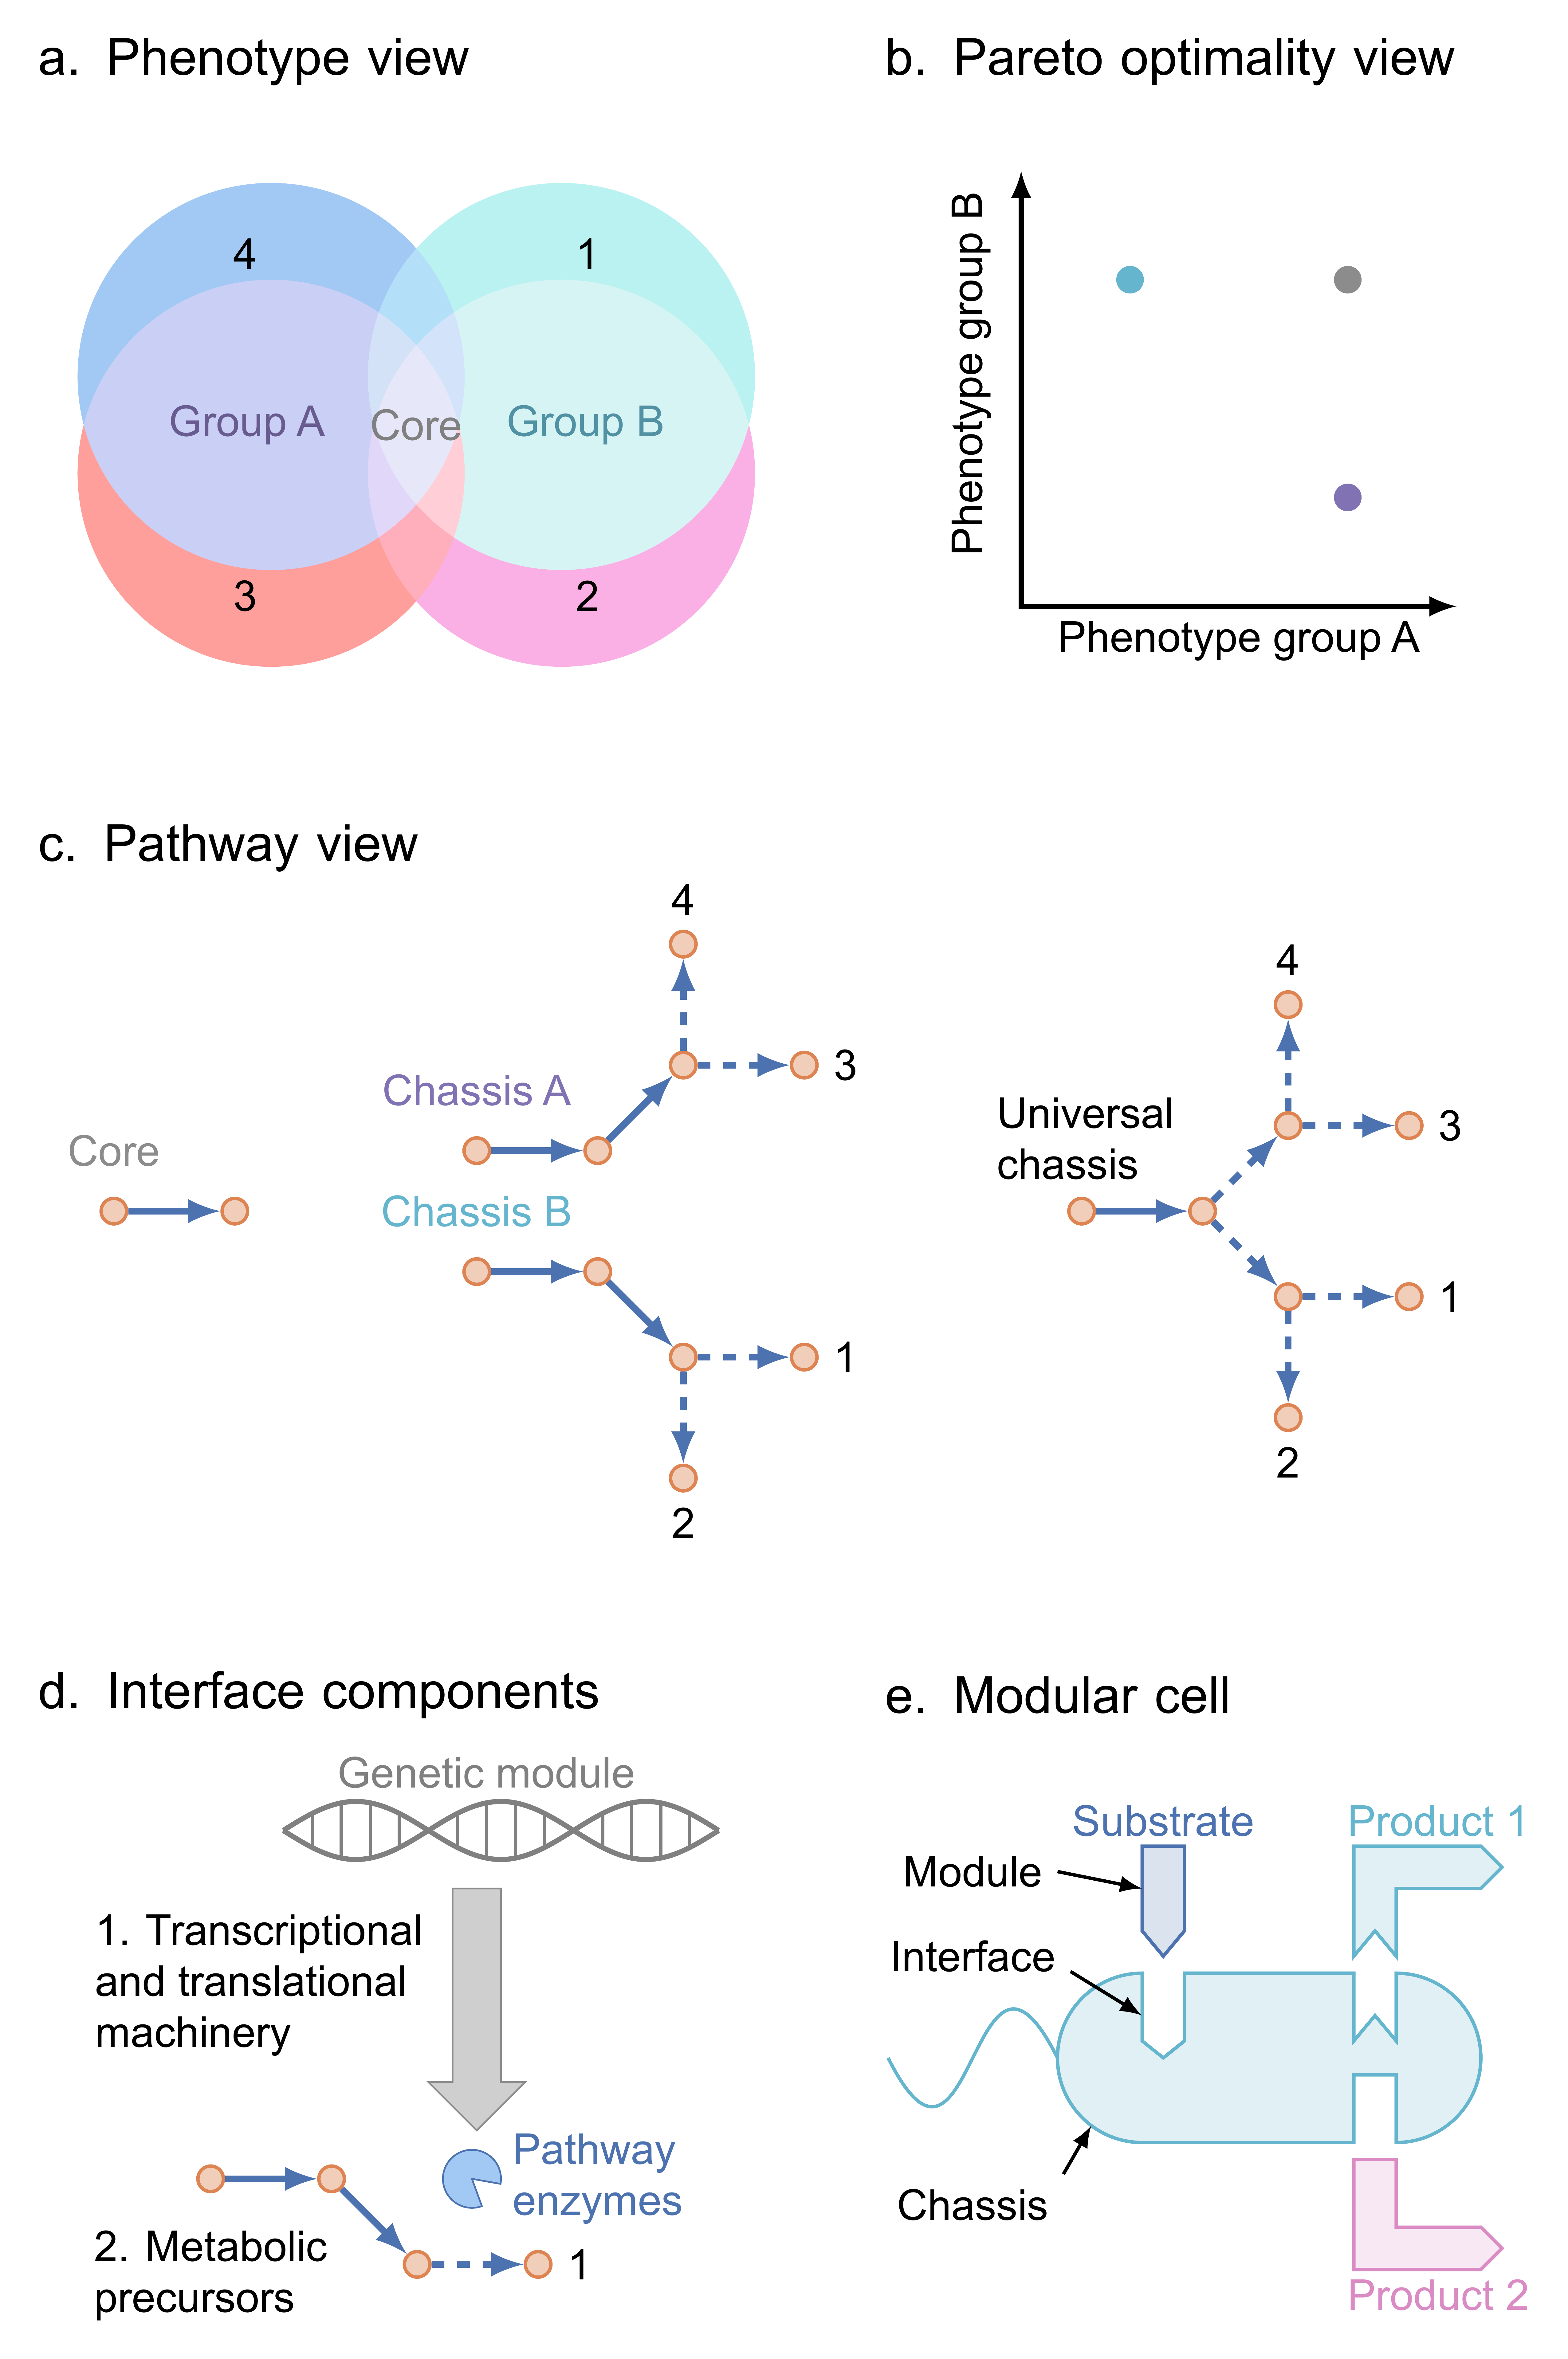
\includegraphics[height=.7\textheight,keepaspectratio]{modcell-concept.png}
    \caption[Modular cell design principles]{Modular cell design principles. (a) Multiple target phenotypes often share common functional states; e.g., different target molecules for overproduction that share precursors and undesired byproducts.
    (b) Several chassis strains are built by optimizing towards different phenotype groups, minimizing the effort required to build modules, at the expense of incompatibility among chassis. Alternatively, a universal core chassis can be build that would require more functions to be performed by the modules, likely introducing undesirable redundancy in module construction.
    (c) In the context of metabolic pathways, modularity can be described in terms of common precursors and downstream pathways.
    (d) The key component of a modular cell system are properly defined interfaces, the chassis must provide adequate enzyme biosynthesis machinery and metabolic precursors for modules to function properly. (e) The proposed modular cell is an efficient chassis strain compatible with modules that enable target phenotypes, minimizing redundant efforts and increasing robustness, hence accelerating the design-build-test cycles in strain engineering.
    }
    \label{fig7:modcell}
\end{figure}

%(Figure~\ref{fig7:modcell}a)
Engineering microbes towards novel phenotypes often repeats previous efforts leading to slower design cycles and less robust systems.
Alternatively, to avoid such redundancy we can design a modular cell chassis that interfaces with a variety of modules (Figure~\ref{fig7:modcell}).\citep{garcia2019, garcia2019b}
The modular cell chassis is built in a top-down manner by removing metabolic functions from a parent strain, then different modules are inserted into the chassis to obtain production strains that optimally display the target phenotype (e.g., high titer, rate, and yield of a given molecule).
Due to the conflicting biochemical requirements of different pathways %, under a limited number of genetic manipulations to construct chassis and modules,
the modular cell design problem was formulated as the following multi-objective optimization problem (MOP) known as ModCell2\citep{garcia2019}, which is summarized as follows:


\begin{alignat}{3}
    & \underset{ \; y_j, z_{jk}}{\max} \quad (f_1, f_2, \ldots, f_{|\mathcal{K}|})^T \quad \text{s.t.}  \label{eq7:of1} \\
    &  \quad f_k \in \, \text{arg }\underset{}{\text{max}} \Bigg\{ \frac{1}{f_k^{max}}\sum_{j \in \mathcal{J}_k} c_{jk}  v_{jk} \quad \text{s.t.} \label{eq7:of2}\\
    & \quad \qquad \sum_{j\in \mathcal{J}_k}S_{ijk}v_{jk} = 0 && \text{for all } i \in \mathcal{I}_k  \label{eq7:mb}\\
    & \quad \qquad  l_{jk} \le v_{jk} \le u_{jk}  && \text{for all } j \in \mathcal{J}_k \label{eq7:rb}\\
    & \quad \qquad  l_{jk} d_{jk} \le v_{jk} \le u_{jk} d_{jk} && \text{for all } j \in \mathcal{C} \label{eq7:db}\\
    & \quad \qquad \; d_{jk} = y_j \lor z_{jk} \; \Bigg\} && \text{for all } k \in \mathcal{K} \label{eq7:defdjk} \\
    & \quad z_{jk}\le (1-y_j) && \text{for all } j \in \mathcal{C}, \, k \in \mathcal{K} \label{eq7:mr1}\\
    & \quad \sum_{j \in \mathcal{C}}z_{jk} \le \beta && \text{for all } k \in \mathcal{K} \label{eq7:mr2} \\
    & \quad \sum_{j \in \mathcal{C}} (1-y_j) \le \alpha \label{eq7:a}
\end{alignat}

\noindent This MOP simultaneously maximizes all objectives $f_k$ \eqref{eq7:of1}, where $k$ belongs to the set of production networks $\mathcal{K}$.
Each production network represents the combination of the chassis with a specific production module, and it is simulated through a stoichiometric model\citep{palsson2015} (\ref{eq7:of2}-\ref{eq7:defdjk}) with a set of metabolites $\mathcal{I}_k$ and a set of reactions $\mathcal{J}_k$.
The stoichiometric model predicts metabolic fluxes according to the following constraints:
(i) mass-balance \eqref{eq7:mb}, where $S_{ijk}$ represents the stoichiometric coefficient of metabolite $i$ in reaction $j$ of production network $k$, (ii) flux bound \eqref{eq7:rb} that determine reaction reversibility and available substrates, where $l_{jk}$ and $u_{jk}$ are lower and upper bounds respectively, and (iii) genetic manipulation \eqref{eq7:db}, i.e., deletion of a reaction $j$ in the chassis through the binary indicator $y_{j}$, or insertion of a reaction $j$ in a specific production network $k$ through the binary indicator $z_{jk}$.
Only a subset of all metabolic reactions, $\mathcal{C}$, are considered as candidates for deletion, since many of the reactions in the metabolic model cannot be manipulated to enhance the target phenotype.

The desirable phenotype $f_k$ for production module $k$ is determined based on key metabolic fluxes $v_{jk}$ (mmol/gDCW/h) predicted by the model (\ref{eq7:of2}-\ref{eq7:db}).
For this study we selected the weak growth coupled to product formation (\emph{wGCP}) design objective that requires a high minimum product synthesis rate at the maximum growth-rate, enabling growth selection of optimal production strains.
Hence, in \emph{wGCP} design, the inner optimization problem seeks to maximize growth rate while calculating the minimum product synthesis rate through the linear objective function \eqref{eq7:of2} (where {$c_{jk}$ is $1$ and $-0.0001$ for $j$ corresponding to the biomass and product reactions across all networks $k$, respectively, and 0 otherwise).
In general, the definition of $f_k$ need not be linear and other design phenotypes can be defined.\citep{garcia2019}

Finally, design constraints (\ref{eq7:mr1}-\ref{eq7:a}) define the limitations of the design variables representing genetic manipulations, $y_j$ and $z_{jk}$.
As part of modular cell design, reactions can be removed from the chassis but inserted back to specific production modules, enabling the chassis to be compatible with a broader number of modules \eqref{eq7:mr1}.
The total module reaction additions and reaction deletions in the chassis are limited by parameters $\beta$ \eqref{eq7:mr2} and $\alpha$ \eqref{eq7:a}, respectively.%, to avoid unnecessary genetic manipulations that are generally time-consuming to implement and can lead to unforeseen phenotypes.


\subsection{Solution techniques for multi-objective optimization problem}
% All this info is background/lit reveiw, but it seems to fit better in its own section than in the intro
% - Define Pareto optimality
% - Explain why we choose MOEA instead of MILP? <= Is this a method?
% - Explain how MOEA works for next section (how important is this?)

Without loss of generality, consider a multi-objective optimization problem with design variables $x$ from a set $\mathcal{X}$ and objective functions $f_i(x)$:
\begin{equation*}
    \underset{ \;x}{\max} \quad F(x) = (f_1(x), f_2(x), \ldots)^T \; \forall x \in \mathcal{X}
\end{equation*}
The solution of such optimization problem is denoted as Pareto set:
\begin{equation*}
    \mathcal{PS}:=\{x \in \mathcal{X}:\nexists \, x' \in \mathcal{X}, F(x') \prec F(x)\} \label{eq7:ps}
\end{equation*}
Here $F(x') \prec F(x)$ indicates that the objective vector $F(x')$ \emph{dominates} $F(x)$, defined as $f_i(x') \ge f_i(x)$ for all objectives $i$, and $f_i(x') \ne f_i(x)$ for at least one $i$. Hence, the Pareto set contains all non-dominated solutions to the optimization problem, i.e., when comparing any two non-dominated solutions, the value of a certain objective must be diminished in order to increase the value of a different objective. The projection of the Pareto set on the objective space is denoted Pareto front: %This can be easily visualized in the Pareto front, defined as the projection of the Pareto set in the objective space: %TODO: Let the reader know why PF is useful? Since it is referenced later
\begin{equation*}
    \PF:=\{F(x): x \in \mathcal{PS} \}
\end{equation*}

MOP can be solved either directly or by conversion into a single-objective problem.\citep{marler2004}  When solved directly, multi-objective evolutionary algorithms (MOEA) are often used to identify the Pareto set, then the designer selects interesting solutions.
On the other hand, when the problem is converted into a single-objective optimization problem, this requires some form of \textit{a priori} specification of preference towards desired Pareto optimal points.
The main advantage of the second approach is that single-objective problems are easier to solve and powerful algorithms such as branch and bound used for mixed-integer linear programing (MILP) are available. % (Note: The state of the art solvers use also cutting planes and other heuristics on top of branch and bound. So I feel that branch and bound is not accurate enough  to later refer to it as the MILP solving method.)
Briefly, MOEA are population based heuristics where potential solutions are iteratively modified based on stochastic processes and information from other potential solutions to identify better solutions, while MILP solver algorithms systematically partition the design space to efficiently identify optimal solutions.
Both approaches have been successfully applied to design modular cells for problems with up to 20 objectives.\citep{garcia2019, garcia2019c, garcia2019d}
MILP can guarantee solution optimality, unlike MOEA. However, effective MILP solver algorithms remain highly challenging to parallelize. \citep{ralphs2016} % Also consider citing (can a million cores solve a ILP?)
Therefore, MOEA presents better options to address problems with many-objectives through high-performance computing as discussed next.

\subsection{Implementation of high-performance parallel many-objective evolutionary algorithm}
% - Describe master-slave vs island, why island is necessary, and other details that might be relevant in the implementation?
% - Define computing processes
% - The basics of genetic algorithms seem to have been introduced to late?
% - Explain any necessary background to understand the benchmarking results.
% - Important: Parameters need to be defined here to follow benchmarking discussion. Even easier, create a table that defines parameters.
% - Note MOEA are described above

The original ModCell2 implementation \citep{garcia2019, garcia2019c} is compatible with several MOEA and used a master-slave parallelization scheme, where the objective functions are evaluated in parallel by slave processes, but every other step in the algorithm is performed serially (Figure~\ref{fig7:algorithm}~a).
This approach contains many serial steps, limiting the scalability of the algorithm with the number processes according to Ahmdal's law.\citep{hill2008}
%In particular for one of the best performing algorithms NSGA-II time complexity \citep{garcia2019c}
In particular, large population sizes, an effective strategy to deal with many objectives,\citep{garcia2019c,ishibuchi2009} can dramatically slow down serial algorithm operations such as non-dominated sorting in NSGA-II, \citep{deb2002} one of the best performing algorithms to solve ModCell2.\citep{garcia2019c}%, quickly turning the serial part into a major performance bottleneck.


\begin{figure}[h]
    \centering
    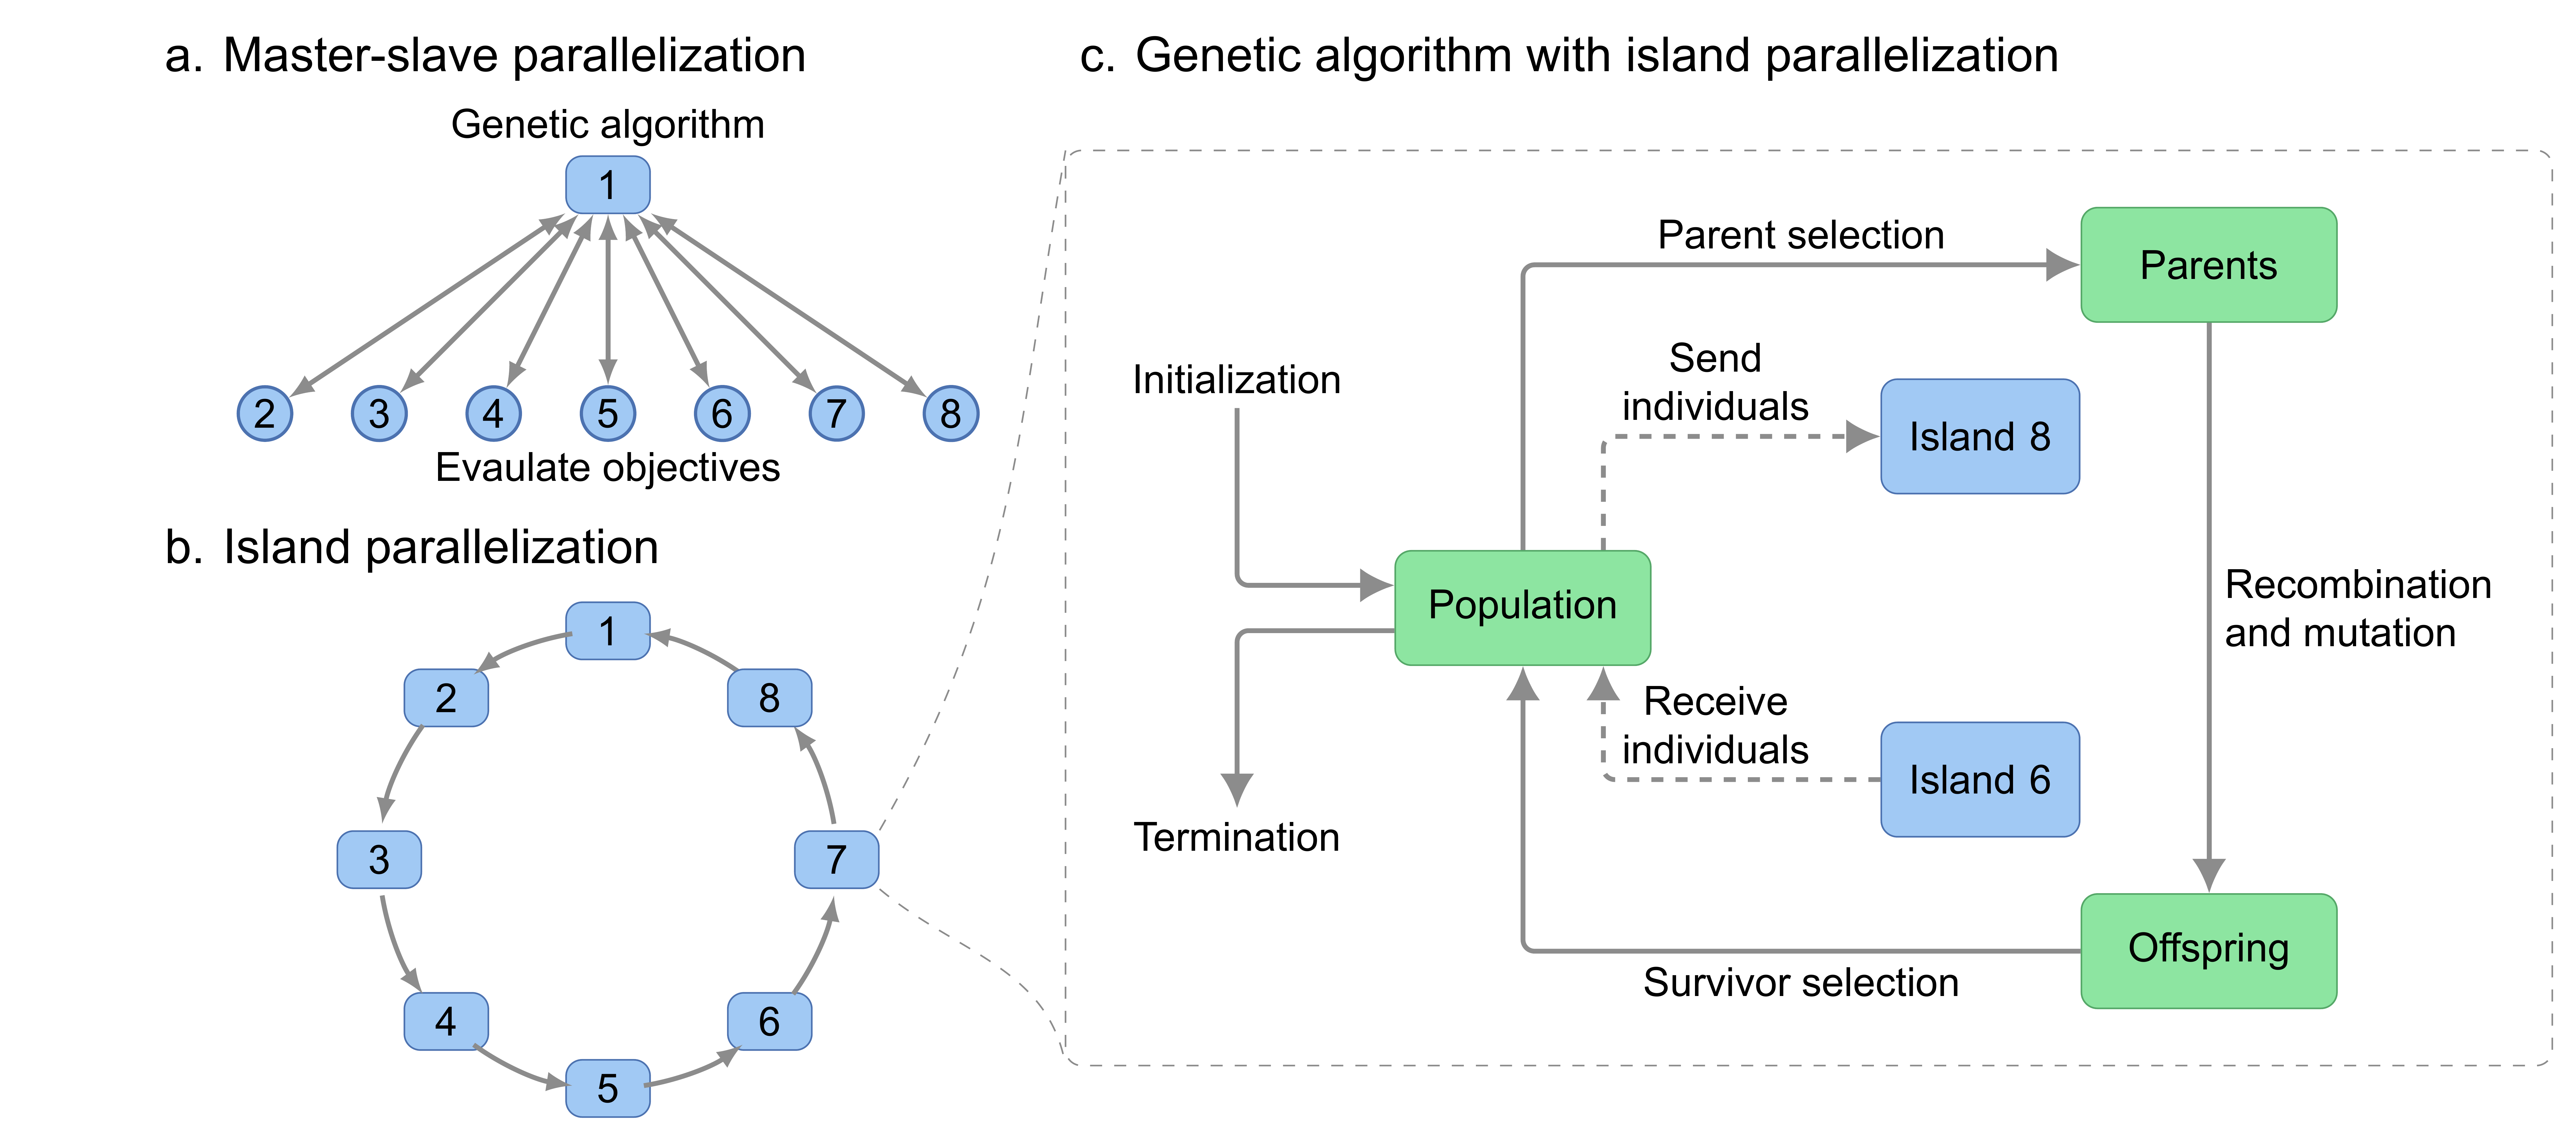
\includegraphics[width=\textwidth,keepaspectratio]{algorithm.png}
    \caption[Parallelization schemes for multi-objective evolutionary algorithm]{Parallelization schemes for multi-objective evolutionary algorithm. (a) Master-slave approach used in the original ModCell2 implementation. (b) Island parallelization following ring topology implemented in ModCell-HPC. (c) Key steps in evolutionary algorithm.} %TODO balance info here with text descritipon, but make the figure standalone. Provide brief ga description of part c, in particular describe the meaning of the words used in the figure.
    \label{fig7:algorithm}
\end{figure}

%An effective strategy to deal with many objectives is to use large
%In particular, for large populations sizes, an effective strategy to deal with large numbers of objectives, \citep{garcia2019c,ishibuchi2009},  certain algorithm steps like non-dominated population sorting in NSGA-II,\citep{deb2002} one of the best performing algorithms to solve ModCell2,\citep{garcia2019c}, quickly turning the serial part into a major performance bottleneck.

To overcome the issues of the master-slave approach, we implemented an island parallelization scheme, where each computing process is an instance of the MOEA (Figure~\ref{fig7:algorithm}~b).
These instances exchange individuals (i.e., potential solutions) in a process called migration, which enhances overall convergence towards optimal solutions (Figure~\ref{fig7:algorithm}~c).
The migration operation allows for multiple configurations that reflect which individuals are exchanged and how such exchange happens.
These options are captured by the migration type and migration interval parameters, respectively (Table~\ref{tab7:parameters}).
To enhance performance and scalability, the migration process was implemented asynchronously, i.e., the population within each island can continue to evolve without needing to wait for sent individuals to arrive at their destination island or for incoming individuals to be received.

The software implementation of the proposed island-MOEA, denoted \textit{ModCell-HPC}, is written from the bottom up in the C programming language and available in Supplementary~Material~\ref{sm:code} and \url{https://github.com/TrinhLab/modcell-hpc}.

%This migration process can occur in differentThe number of iterations in between migrations is denoted, \textit{migration frequency}
%A genetic algorithm is an iterative process where a population of potential solutions is modified under heuristic rules in order to identify solutions closer to optimality (Figure~\ref{fig7:algorithm}~c). In the island parallelization scheme, after a certain number of iterations, determined by the \textit{migration frequency}, individuals are sent and received to and from neighboring islands.
%(Table~\ref{tab7:parameters})

%In a genetic algorithm, a population composed by individuals that represent problem variables, is used to produce an offspring by stochastic combinations of their design variables and subsequent evaluation of their fitness (i.e., the design objectives of the optimization problem).


% \item The Matlab implementation of ModCell2 is slow and cannot handle large-scale problems due to both its inability to effectively parallelize beyond a few cores and its inefficient use of CPU and memory resources.
% \item modcell-hpc was written from the bottom up in C and uses MPI to implement island parallelization. In this approach multiple instances of the algorithm run in individual processes known as islands. These islands exchange individuals with certain periodicity in a process called migration.
% \item Migration occurs asynchronously so islands may continue to evolve while messages are being passed, greatly enhancing performance.
% \item This approach can potentially scale to hundredths or thousands of cores since the program does not contain any sequential operations that would become a bottleneck (See Amdahl's Law).

\subsection{Computation hardware}
We conducted all ModCell-HPC computations in \emph{beacon} nodes from the Advanced Computing Facility at the Joint Institute for Computational Science (The University of Tennessee and Oak Ridge National Laboratory). Each node contains a 16 core Intel Xeon E5-2670 central processing unit (CPU) and 256 GB of random access memory (RAM). The results were analyzed in a desktop computer with an Intel Core i7-3770 CPU and 32 GB of RAM.

\subsection{Target product identification}
The target products are endogenous \textit{E. coli} metabolites that meet the following requirements: i) Maximum theoretical yield above 0.1 (mol product/mol of substrate); ii) organic; iii) can be coupled to growth under anaerobic conditions, indicated by the existence of a constrained Minimal Cut Set (cMCS) with yield above 50\% under anaerobic conditions in a previous study;\citep{kamp2017} iv) If the same metabolite appears in multiple compartments, only one instance is selected, prioritizing extracellular, then periplasm, then cytosol.
This resulted in 161 target metabolites.
Metabolites that did not have a secretion mechanism originally present in the model required to add an exchange pseudo-reaction that represents metabolite secretion to the growth medium or intracellular accumulation at steady-state. %TODO: Not sure where to mention this, or if very relevant at all.
The products in the resulting library have diverse molecular weights and are highly reduced due to the use of anaerobic conditions (Figure~\ref{fig7:biochemical-properties}).

%If the same metabolite

% Either explain in the table or on the text but avoid redundancy
%The target products are endogenous \textit{E. coli} metabolites that have the potential to be produced in a growth-couple manner according to a previous study by Kamp and Klamt.\citep{kamp2017}
%We further filtered the target products according to the criteria of Table \ref{tab7:products}.
%In summary, only endogenous metabolites that are organic, have a maximum theoretical yield above 0.1 (mol product / mol of substrate) and can potentially be coupled to growth under anaerobic conditions were kept as targets.

\subsection{Model configuration}
Since the study of Kamp and Klamt\citep{kamp2017} was used as basis to identify products compatible with growth-coupled design, we used the same model configuration, adapted to the most recent \textit{E. coli} model iML1515.\citep{monk2017} Briefly, glucose uptake limit was set to 15 (mmol/gCDW/h); the default ATP maintenance value in iML1515 was used; 20\% of the maximum anaerobic growth rate was used as the minimum growth rate, corresponding to 0.0532 (1/h). The model configuration is equivalent to previous modular cell design studies\citep{garcia2019} except for the higher glucose uptake rate.

%The only difference between anaerobic and aerobic model configurations is the oxygen uptake rate limit, which is 0 in the former and 20 mmol/gCDW/h in the later.

\subsection{Solution improvement process}
The MOEA output can be improved by: i) eliminating \emph{futile module reactions}, i.e., module reactions that when removed do not diminish the objective value of the associated production network; and ii) coalescing module reaction, i.e., in multiple designs with the same deletions, but different module reactions, can often be combined to obtain a superior solution. This procedure is detailed in Figure~\ref{fig7:processing}.
%We applied this improvement process to anerobic and aerobic results and observed remarkable improvement in solution quality. (most module reactions are futile, the PF of $\alpha=5,\beta=1$ has a minimal set cover of 8 before coalescing and 3 after coalescing.
% NOTE: This was not applied to benchmarking, but was applied to all other solutions.

\subsection{Design characterization} \label{sec:design_characterization}
\subsubsection{Compatible modules and compatibility}
An important qualitative feature of a designed chassis is module compatibility.
A chassis and a given module are \emph{compatible} if the performance of such module is above a defined threshold.
In this study, we used the \textit{wGCP} design objective that corresponds to the minimum product yield at the maximum growth rate, and selected a threshold of 0.5 to establish compatibility. Under these conditions, we expect a module compatible with the chassis can lead to a product yield above 50\% of the theoretical maximum during the growth phase.
The \emph{compatibility} of a chassis corresponds to the number of modules that are compatible with it.

\subsubsection{Minimal covers} \label{sec:minimal_covers}
After solving the modular cell  design problem, we obtain several Pareto optimal chassis, $h \in \mathcal{H}$, that are compatible with different subsets of products. %I.e., a design $h$ is said to be compatible with product $k$, if its objective function is above a defined threshold.
A set cover is a collection of designs $h$ such that their union contains all compatible products.
Hence, we developed minimal set cover analysis to find the smallest number of designs needed to ensure all compatible products are present in at least one of the designs.
This is formulated as the canonical minimal set covering problem of integer programming:

\begin{align}
    & \underset{ \;x_h \in \{0,1\}}{\min} \sum_{h \in \mathcal{H}} ( \gamma_h x_h) \label{eq7:mc_1}\\
    & \nonumber \; \text{subject to:} \\
    & \quad \sum_{h \in \mathcal{H}} a_{hk} x_h \ge 1 & \forall \; k \in \mathcal{K'} \label{eq7:mc_2}%\\
    %& \quad x_h \in \{0,1\} & \forall h \in \mathcal{H} \label{eq7:mc_3}
\end{align}

\noindent
The optimization problem minimizes the number of designs in the set cover \eqref{eq7:mc_1}.
The binary indicator variable $x_h$ takes a value of 1 if design $h$ is selected as part of the cover and 0 otherwise.
Certain designs can be prioritized (e.g., due to the genetic manipulations they contain being preferable or to reduce the number of alternative solutions) using the weighting parameter $\gamma_h$, however in all our simulations we set $\gamma_h = 1$. All compatible products $k$ must be included in at least one of the selected designs \eqref{eq7:mc_2}. The parameter $a_{hk}$ takes a value of 1 if product $k$ is compatible with design $h$ and 0 otherwise. There must exist at least one $h \in \mathcal{H}$ for which $a_{hk} = 1$ to ensure a feasible solution exists, hence $\mathcal{K'}$ is the set of products compatible in at least one design of the Pareto front.
%Thus if a product is not compatible at all under the specified modcell design parameters ($\alpha$ and $\beta$) it must be discarded from $\mathcal{K'}$ or the problem would become infeasible.

To enumerate all minimal covers we iteratively solved the minimal cover problem (\ref{eq7:mc_1}-\ref{eq7:mc_2}) with the addition of an integer cut inequality \eqref{eq7:ic} in each iteration that removes a previously found solution $\mathcal{S}$.
\begin{equation}
    \sum_{h\in\mathcal{S}} x_h \le |\mathcal{S}|  - 1 \label{eq7:ic}
\end{equation}
%Here $\mathcal{S}$ is a previously found optimal solution that should be excluded from the problem.


\section{Results}

\subsection{Design of modular \textit{E. coli} platform strains for growth-coupled production}

\paragraph{A small number of genetic manipulations are sufficient for highly compatible chassis}
We tuned ModCell-HPC method parameters (Supplementary Text 1) and used it to design \textit{E. coli} modular cells for our library of 161 products.
%, we used ModCell-HPC to design modular cells.
First, we scanned a broad range of design parameter combinations ($\alpha$-$\beta$: 5-1, 10-2, 20-4, and 40-8) to identify the required genetic manipulations for highly compatible designs (Figure~\ref{fig7:parameter-scan} a).
Increasing the number of genetic manipulations leads to an average increase in design compatibility.
However, the maximum compatibility remains around 50\% of the library (80 products) for all cases.
Indicating that highly compatible platforms can be built with a small number of genetic manipulations.
We selected the designs with case of $\alpha=5,\beta=1$ (Supplementary~Material~\ref{sm:designs}) for further analysis, since designs with fewer genetic manipulations are likely more accurately simulated and also easier to implement in practice.
%We will analyzed overall features of the designs , then focus on specific suggestions for experimental implementation.

\paragraph{A few reaction deletions in central metabolism targeting byproducts and branch-points are relevant to build chassis strains}
% Key points:
% - Few reactions are relevant
% - Reactions are concentrated in central metabolism
% - Reactions belong to two categories: Remove undesired byproducts and metabolic branchpoints
% - Branchpoitns are not commonly targeted, even though their potential importance was highlighted early on:
% https://science.sciencemag.org/content/252/5013/1675
% \citep{stephanopoulos1991}
% the use of models may assist in solving the problem

We sorted reaction deletions according to how often they appear across designs (Table~\ref{tab7:top20deletions}).
The top 7 reactions are used $\ge$10\% of the designs and belong to central metabolism, indicating their importance to accomplish growth coupled to product secretion phenotypes.
%The top 20 reactions mainly belong to central metabolism (Figure~\ref{fig7:deletion-map}), and quickly decay in deletion frequency, highlighting the relevance of the top 3 reactions, appearing in >40\% of the designs, to accomplish the target growth coupled to product secretion phenotypes.
% Central metabolism:
% sauer1999
%The top 3 deletions all apear in 40\% or more of the designs.
%However, this frequency quickly decays.
%Indicating that these reactions, ALCD2x, TPI, and ACALD, are key deletions for growth-coupled product synthesis.
%Both ALCD2x and ACALD are involved in the conversion of acetyl-CoA to ethanol, which is the main pathway for acetyl-CoA reduction and secretion under anaerobic conditions. Unsuprisingly this pathway must be avoided to couple target molecule secretion to growth.
Overall, the role of these deletions can be classified into two functions: i) To eliminate major byproducts; ii) to alter key branch-points in metabolism that influence the pools of precursor metabolites (including carbon, redox, and energy precursors).
% and overall energy efficiency of catabolism.
The first type is generally intuitive and often used in metabolic engineering efforts.\citep{winkler2015}
The second type are not commonly identified unless metabolic model simulations are used, \citep{tokuyama2014, venayak2018, chemler2010}
even though the importance of targeting metabolic branch-points was noted early. \citep{stephanopoulos1991}
%importance of manipulating key metabolic branch-points that are not part or directly upstream of the production pathway was noted early.\citep{stephanopoulos1991}
% - Branchpoitns are not commonly targeted, even though their potential importance was highlighted early on:
% \citep{stephanopoulos1991}
Examples of the later manipulations are TPI deletion, that activates the methylglyoxal bypass,\citep{fong2006} reducing the overall ATP yield resulting from glucose conversion into pyruvate.
Lower ATP yield limits biomass formation hence redirecting carbon flow towards products of interest.
While such strategies are not common, TPI deletion predicted by model simulations was successfully used for enhanced 3-hydroxypropionic acid production,\citep{tokuyama2014} and ATP waisting is receiving increased attention to enhance production of certain molecules.\citep{boecker2019} %NOTE: MAybe ATP waistin is a bit of a strech here?
Another example of branch-point manipulation is PPC deletion, that has been shown to lower flux from lower glycolysis towards the TCA cycle,\citep{de2006,peng2004} resulting in lower succinate production, and an increased pool of \textit{pep}, pyruvate and acetyl-CoA.
Additionally, PPC deletion to increase the \textit{nadph} pool for production of flavonoids was predicted by model simulation and experimentally validated. \citep{chemler2010}
%which synthesis important precursors and also enables succinate secretion. %\citep{} %see MILP paper for succinate citations
In summary, design of highly compatible chassis strains requires not only major byproduct removal, but also manipulation of key branch points in central metabolism.

\begin{table}[ht]
    \caption[Top 20 reaction deletions]{Top 20 reaction deletions for design parameters $\alpha=5$, $\beta=1$ with 162 designs. Counts indicates the percentage of designs where the deletion is used. All reaction and metabolite abbreviations used in this study correspond to BiGG identifiers (\protect\url{http://bigg.ucsd.edu}).}
    \centering
    \resizebox{1\textwidth}{!}{%
\rowcolors{2}{gray!25}{white}
\begin{tabular}{llll}
\toprule
ID	&	Name	&	Formula	&	Counts (\%) \\
\midrule
ALCD2x	&	Alcohol dehydrogenase (ethanol)	&	etoh\_c + nad\_c $\leftrightarrow$ acald\_c + h\_c + nadh\_c	&	57.4	\\
TPI	&	Triose-phosphate isomerase	&	dhap\_c $\leftrightarrow$ g3p\_c	&	45.1	\\
ACALD	&	Acetaldehyde dehydrogenase (acetylating)	&	acald\_c + coa\_c + nad\_c $\leftrightarrow$ accoa\_c + h\_c + nadh\_c	&	40.7	\\
FLDR2	&	Flavodoxin reductase (NADPH)	&	2.0 flxso\_c + nadph\_c $\rightarrow$ 2.0 flxr\_c + h\_c + nadp\_c	&	24.1	\\
PPC	&	Phosphoenolpyruvate carboxylase	&	co2\_c + h2o\_c + pep\_c $\rightarrow$ h\_c + oaa\_c + pi\_c	&	21.6	\\
TKT2	&	Transketolase	&	e4p\_c + xu5p\_\_D\_c $\leftrightarrow$ f6p\_c + g3p\_c	&	15.4	\\
LDH\_D	&	D-lactate dehydrogenase	&	lac\_\_D\_c + nad\_c $\leftrightarrow$ h\_c + nadh\_c + pyr\_c	&	13	\\
G3PD2	&	Glycerol-3-phosphate dehydrogenase (NADP)	&	glyc3p\_c + nadp\_c $\leftrightarrow$ dhap\_c + h\_c + nadph\_c	&	7.4	\\
POR5	&	Pyruvate synthase	&	coa\_c + 2.0 flxso\_c + pyr\_c $\leftrightarrow$ accoa\_c + co2\_c + 2.0 flxr\_c + h\_c	&	7.4	\\
ACKr	&	Acetate kinase	&	ac\_c + atp\_c $\leftrightarrow$ actp\_c + adp\_c	&	6.8	\\
THD2pp	&	NAD(P) transhydrogenase (periplasm)	&	2.0 h\_p + nadh\_c + nadp\_c $\rightarrow$ 2.0 h\_c + nad\_c + nadph\_c	&	6.2	\\
GLUDy	&	Glutamate dehydrogenase (NADP)	&	glu\_\_L\_c + h2o\_c + nadp\_c $\leftrightarrow$ akg\_c + h\_c + nadph\_c + nh4\_c	&	5.6	\\
ASPT	&	L-aspartase	&	asp\_\_L\_c $\rightarrow$ fum\_c + nh4\_c	&	5.6	\\
ASNS2	&	Asparagine synthetase	&	asp\_\_L\_c + atp\_c + nh4\_c $\rightarrow$ amp\_c + asn\_\_L\_c + h\_c + ppi\_c	&	4.9	\\
CBMKr	&	Carbamate kinase	&	atp\_c + co2\_c + nh4\_c $\leftrightarrow$ adp\_c + cbp\_c + 2.0 h\_c	&	4.3	\\
RNDR4	&	Ribonucleoside-diphosphate reductase (UDP)	&	trdrd\_c + udp\_c $\rightarrow$ dudp\_c + h2o\_c + trdox\_c	&	3.7	\\
RPE	&	Ribulose 5-phosphate 3-epimerase	&	ru5p\_\_D\_c $\leftrightarrow$ xu5p\_\_D\_c	&	3.1	\\
SERD\_L	&	L-serine deaminase	&	ser\_\_L\_c $\rightarrow$ nh4\_c + pyr\_c	&	3.1	\\
LCARS	&	Lacaldehyde reductase (S-propane-1,2-diol forming)	&	h\_c + lald\_\_L\_c + nadh\_c $\leftrightarrow$ 12ppd\_\_S\_c + nad\_c	&	2.5	\\
FUM	&	Fumarase	&	fum\_c + h2o\_c $\leftrightarrow$ mal\_\_L\_c	&	2.5\\
\hline
\end{tabular}}

    \label{tab7:top20deletions}
\end{table}

%PPC
%TKT2
% TKT1 overxpression is imnportant for aromatic aminoacids and other products

% This paper as ppc and tpi deletion, though just examined in the context of evolution:
% https://www.nature.com/articles/ng1432

%Notably the actitivty of this gene, w.... evolved mutants. Highlighting that special care must be t... for underground metabolism in growth-coupled design % \citep{wilbanks2017}


% Note above flavodoxin dependent
% https://ecocyc.org/ECOLI/NEW-IMAGE?type=ENZYME&object=Flavodoxin
%  These are not commonly paid attention in e.coli, even though they are known to be active (when?). No clear reason why
% In terms of the model FLDR2 for example exchange nadph and fldx then POR5 can oxidize pyruvate using nadph

\paragraph{Module reaction usage reveals pathway interfaces and unbiased module definition}
% Key points:
% - Reminder of module reactions, enhance compatibility
% - We can identify what reactions are critical for certain producst
% - Instead of defining what reactions must be present in a module, this allows to ... Further flux analysis as done previously can also lead to reactions that should be overexpressed.
% - Use the trivial cases first (e.g., acetate, lactate, ethanol) then move on to the more sophisticated pathways/less obvious cases.
The modular cell optimization formulation not only identifies genetic manipulations in the chassis, but also in the production modules.
Module reactions correspond to reactions deleted in the chassis but inserted back in specific production modules to enable compatibility.
We examined the module reactions used by all designs (Figure~\ref{fig7:module-usage}).
As expected, ethanol often uses ALCD2x, acetate uses ACKr, and lactate LDH\_D, all these are the primary producers of those metabolites.
More notably, we observe that products which are not highly reduced such as acetate, use ACALD, and similarly 3-methyl-2-oxobutanotae and 2,3-dihydroxy-3-methylbutanoate (which are naturally precursors of valine and artificially of isobutanol\citep{atsumi2008,atsumi2010}) use FUM and MDH.
These module reactions enable the synthesis of ethanol and succinate, respectively, necessary to maintain electron balance in the production of less reduced metabolites.
Interestingly, fatty acids tend to use TPI, which as mentioned earlier, its deletion activates the methylglyoxal bypass lowering the overall ATP yield.
The first step in fatty acid biosynthesis, acetyl-CoA carboxylase, requires one ATP per mol of malonyl-CoA, explaining the usage of TPI as a module reaction for this family of products.
Overall, module reactions provide with a systematic method to enhance the compatibility of a chassis, leading to more efficient strategies and revealing potential metabolic flux bottlenecks that are not always directly upstream of the target product.


\begin{figure}[h]
    \centering
    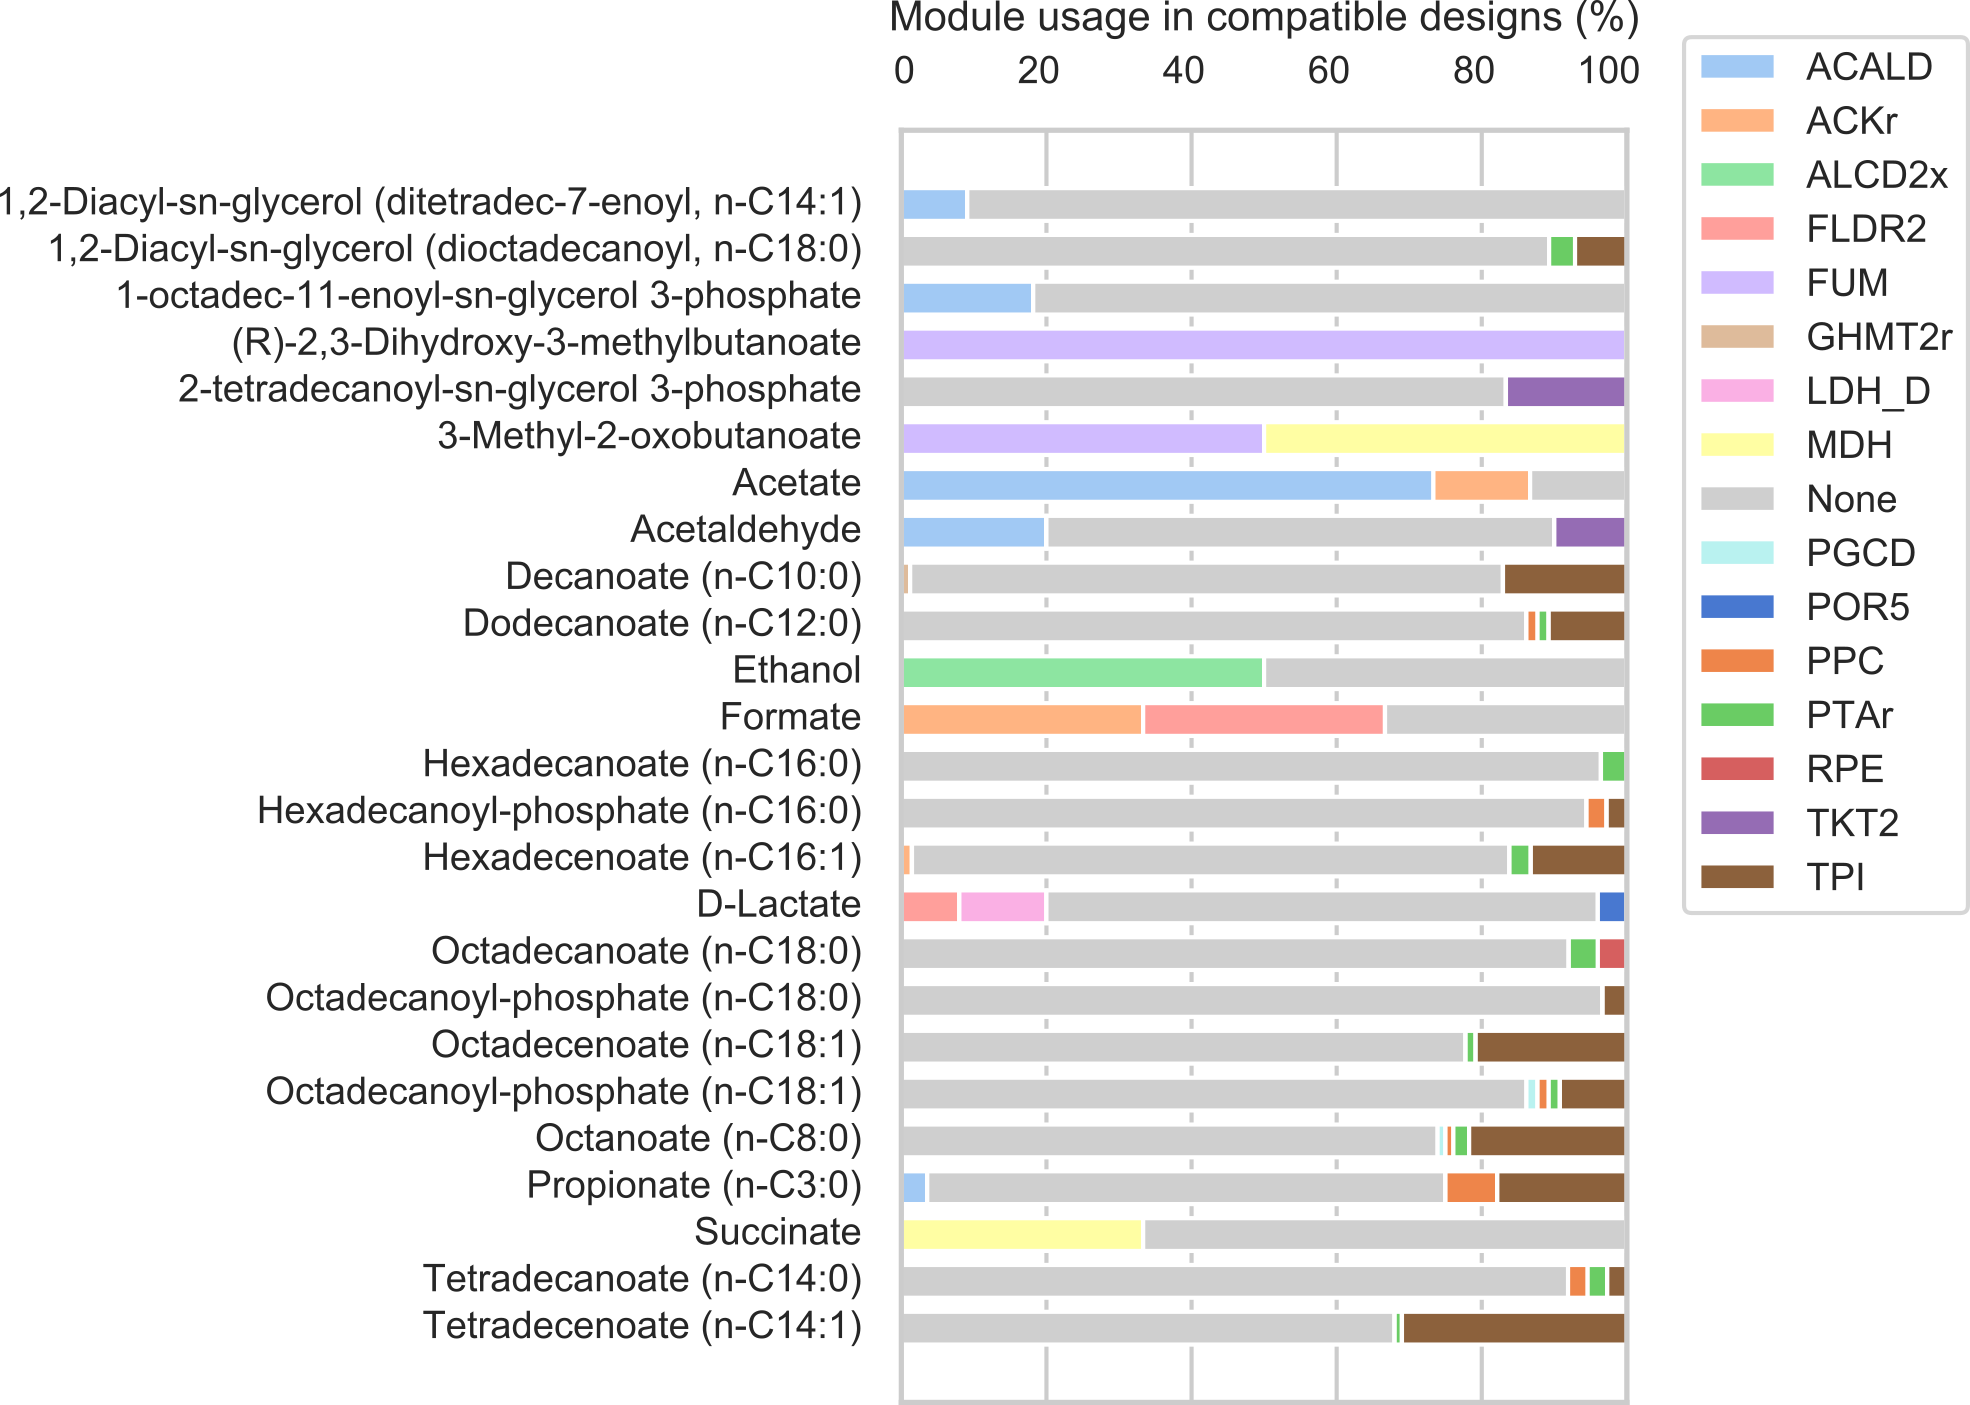
\includegraphics[width=\textwidth,keepaspectratio]{a5_b1_comp_0p5_module_usage.png}
    \caption[Module reaction usage]{Module reaction usage for design parameters $\alpha=5$ and $\beta=1$. Only designs compatible with the product are considered in the module usage frequency.}%For each product, designs in which the product is compatible are selected and the frequency of used module reactions is extracted.}
    \label{fig7:module-usage}
\end{figure}

% Why not many products use module reactions?

\paragraph{Three chassis strains is the smallest set of designs needed to cover all compatible modules}
% Key points:
% - We apply minimal covers to demonstrat the smallest ...
% - We find in this case the minimal cover size is 3, there are xxx, resulting form
One of the tenets of efficient design is to minimize redundant efforts.
When it comes to the construction of platform strains, we would like to identify the smallest set of strains needed to cover a certain product library.  %while avoiding redundancy.
To address this question we use the set of designs produced by ModCell-HPC and a set covering optimization problem (Section~\ref{sec:minimal_covers}).
%We applied this analysis to the set of designs with
For the Pareto set of designs $\alpha=5,\,\beta=1$ we  enumerated a total of 12 minimal covers of size 3. These covers are spanned by combinations of 8 unique designs (Figure~\ref{fig7:cover-graph}). %NOTE: Could add the table with designs
We selected cover k that contains designs 82, 121, and 124, which use few deletions and have similar genetic manipulations among them.
All designs in the cover have in common the deletion of ALCD2x and LDH\_D, disabling production of ethanol and lactate, the major reduced products of anaerobic growth in \textit{E. coli}.
% and well-known targets.
Designs 121 and 124 are compatible with the same 57 products, and design 121 is uniquely compatible with ethanol, formate, and 2,3-dihydroxymethylbutanoate, while design 124 is uniquely compatible succinate (Figure~\ref{fig7:design-comparison} a).
These two designs only differ in that design 121 uses FUM deletion while design 124 uses MDH deletion,
(Figure~\ref{fig7:design-comparison} b)
FUM deletion blocks metabolic flux towards succinate secretion%
%FIXME: this can be contradictory with what I said earlyr about 23dhmb production,
, while MDH routes it toward this product (Figure~\ref{fig7:design-comparison} c).
%Given a few additional genetic manipulations they could potentially be combined. % NOTE: Probably not good to say, since someone might suggest to do it
Design 82 is the only design that features the deletion of FLDR2 and PPC, and it is uniquely compatible with 24 modules, all fatty acids, making this design quite different from from 121 and 124.
FLDR2 is coupled with POR5 to form a pathway for the reduction of pyruvate into acetyl-coa consuming \textit{nadph} (Figure~\ref{fig7:design-comparison} c), a key redox cofactor in fatty acid biosynthesis.
PPC deletion is another strategy to increase \textit{nadph} available that has been experimentally validated. \citep{chemler2010}
Overall, these designs can be efficiently built due to their similarity,  and are composed of strategies that have been demonstrated in isolation but also seem applicable to cover large product families.

\begin{figure}[hp]
    \centering
    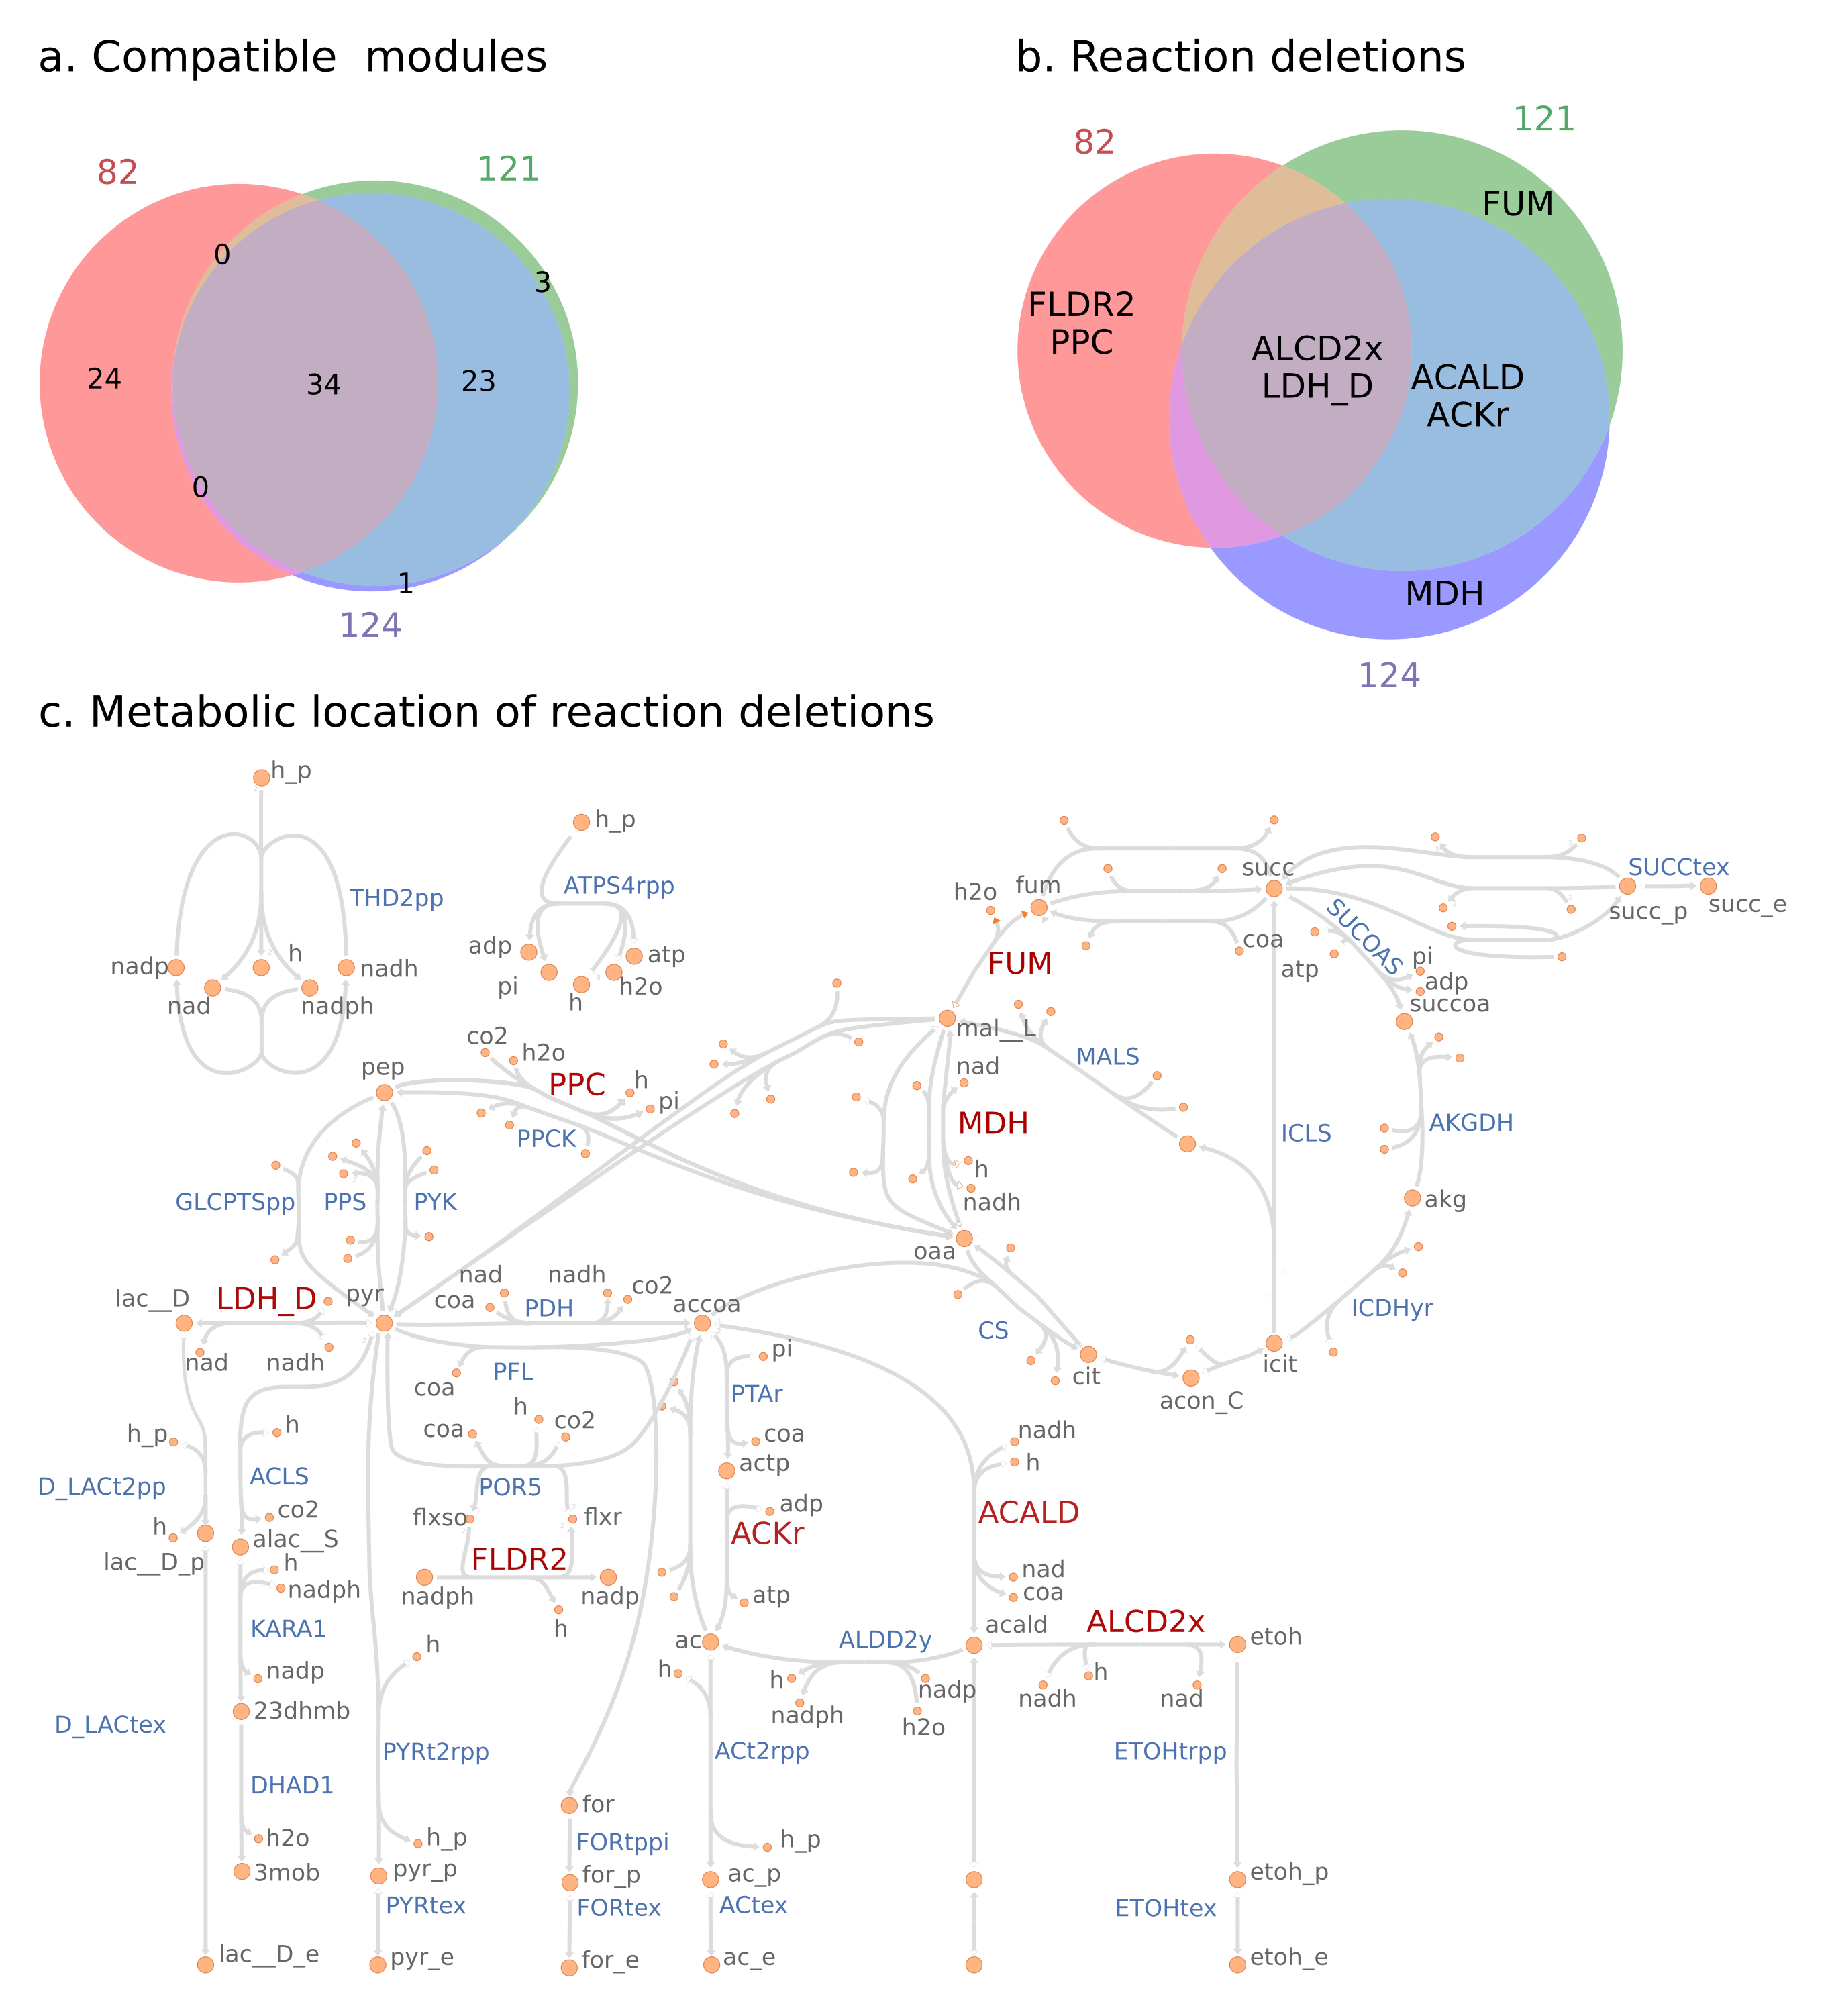
\includegraphics[width=\textwidth,keepaspectratio]{cover-venns.png}
    \caption[Comparison of designs in the selected minimal cover]{Comparison of designs in the selected minimal cover. (a) Venn diagram of products compatible with each design. The products uniquely compatible with specific designs are:
       Design 121: \textit{etoh, for, 23dhmb};
       Design 124: \textit{succ};
%       Design 25: \textit{pe120, 2agpg180, 1ddecg3p, 1agpg180, pgp140, pgp120, pg141, pg140, 2odecg3p, pgp141, ps140, lipidX, 2tdecg3p, ps141, pg120, pe140, 2odec11eg3p, pe141, apg120, ps120, 2hdecg3p, 2hdec9eg3p, pgp161, pg161}.
       Design 82: \textit{pg140, 2hdecg3p, 2odec11eg3p, 1agpg180, pe140, pg161, pg141, 2hdec9eg3p, pgp161, 2agpg180, 1ddecg3p, pg120, pgp141, pgp140, pe141, ps140, apg120, ps120, pgp120, pe120, lipidX, 2tdecg3p, 2odecg3p, ps141}.
    (b) Venn diagram of reaction deletions that constitute each design.
    (c) Metabolic map with reaction deletions colored in red.
       }
    \label{fig7:design-comparison}
\end{figure}


%%%
% Other potential sections:
% - Design for other carbon sources (just repeat analysis but compare key features) or design for unknown modules (identify what "unknown products" are easier to couple, and what designs have the most compatibility with "unknown products"
% - Raise the compatibiliy therhold to e.g., 80. Do more clear product families emerge?

\subsection{Design of modular \textit{E. coli} platform strains for growth-coupled production from various sugar carbon sources} %\subsection{Design of platform strains for other carbon sources}
\paragraph{Non-glucose carbon sources can require more genetic manipulations for high compatibility designs}
We designed modular cells to consume other relevant carbon sources besides glucose also present in feedstocks, including two pentoses, xylose and arabinose, and two more hexoses, galactose and mannose (Figure~\ref{fig7:sugars} a).
For this case study, everything remained the same except for the substrate uptake reaction in the model which was changed to reflect the sole carbon source in each case.
We first scanned the distribution of design compatibilities resulting from various combinations of $\alpha$ and $\beta$ for each carbon source (Figure~\ref{fig7:parameter-scan} b-e).
All cases plateau at maximum compatibilities around 50\%, however, galactose, arabinose and xylose require at least $\alpha=10, \, \beta=2$ to reach this level, while glucose and mannose reach it with only $\alpha=5, \, \beta=1$.
Hence, we selected $\alpha=10, \, \beta=2$ for further analysis.
%Despite the increase in the required number of manipulations,
Overall, this simulation reveals the possibility of highly compatible modular cells for various hexose and pentose carbon sources, at the expense of an increased number of genetic manipulations for some of the carbon sources.

\begin{figure}[hp]
    \centering
    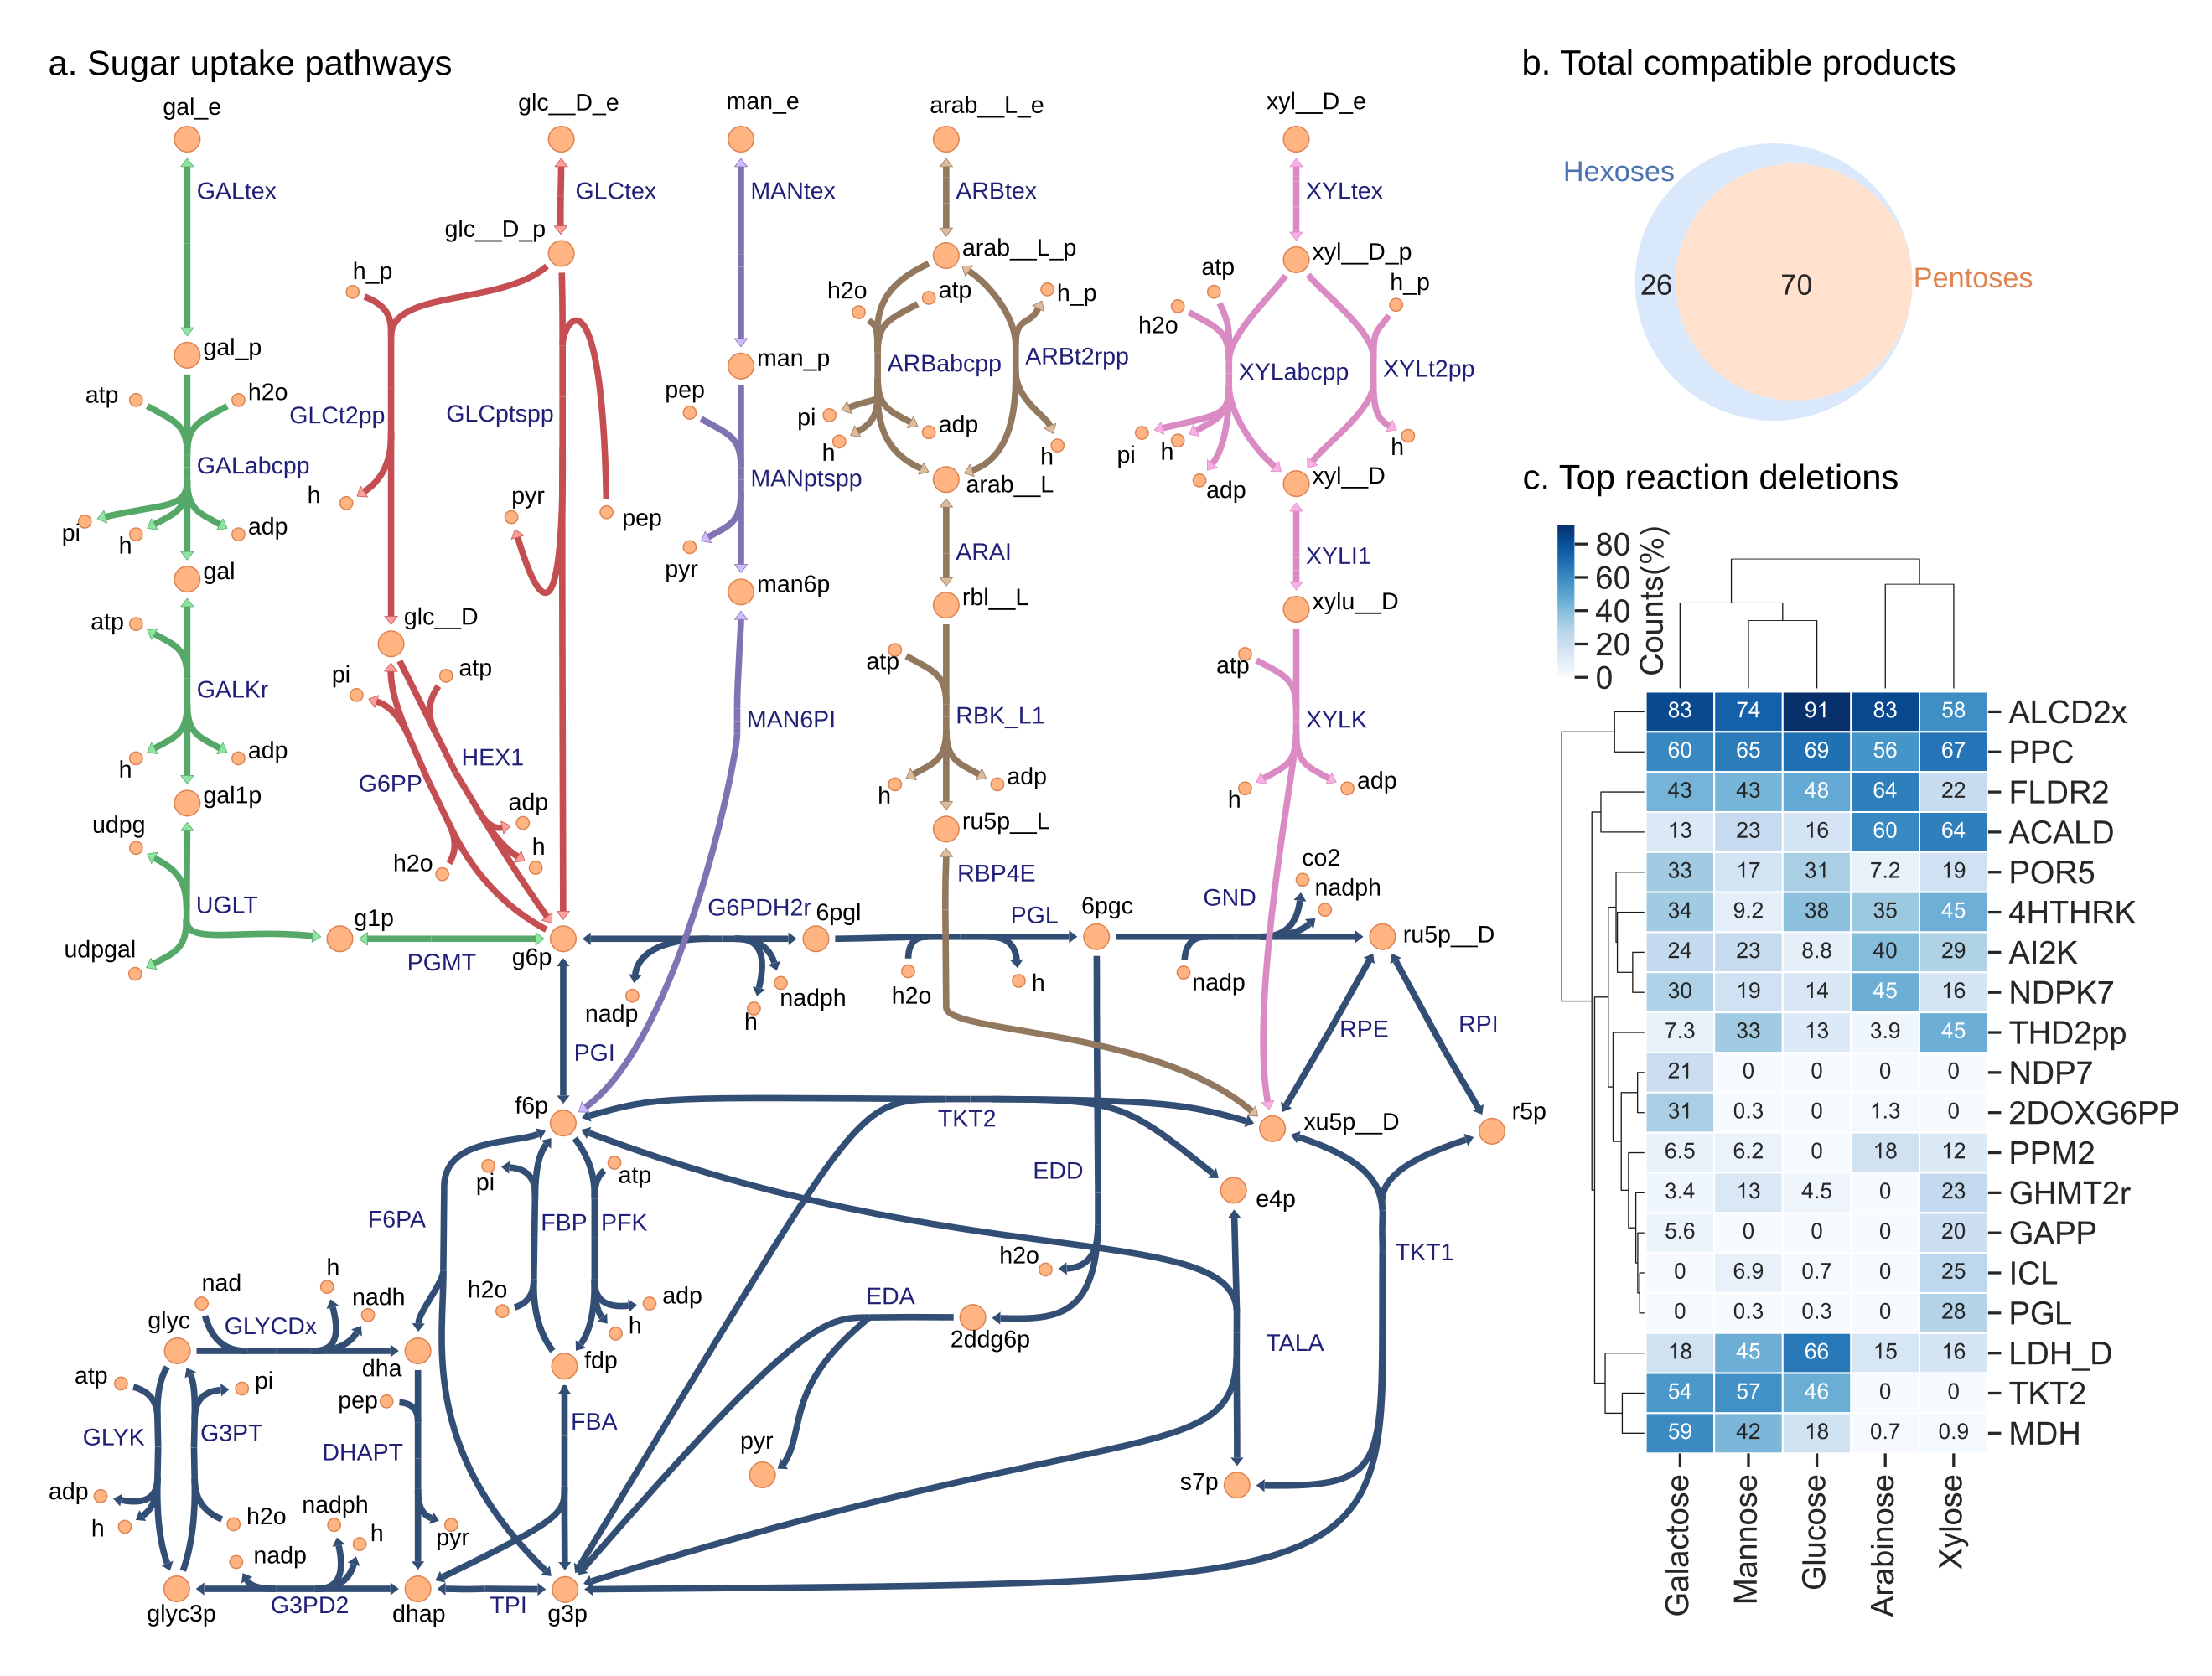
\includegraphics[width=1\textwidth,keepaspectratio]{sugars.png}
    \caption[Design of modular cells for different carbon sources ]{Design of modular cells for different carbon sources with design parameters $\alpha=10, \, \beta=2$. (a) Sugar uptake, pentose phosphate, Entner-Doudoroff, and upper glycolysis pathways. (b) Venn diagram of total products compatible with designs under pentoses and hexoses.
    The 26 products uniquely compatible with hexoses are:
    1agpg180, 2tdecg3p, 2agpg181, 3c3hmp, 3mob, 2hdecg3p, pe141, ps120, 1agpg160, 2agpg160, 23dhmb, ps141, 1agpe180, 2agpg180, apg120, 2agpe180, pe120, 2odec11eg3p, 4mop, lipidX, 3c2hmp, 2ippm, 2hdec9eg3p, 1agpg181, dha, 2odecg3p.
    (c) Top 20 reaction deletions according to deletion frequencies average across carbon sources. The counts for each carbon source correspond to the percentage of designs containing that reaction deletion.}
    \label{fig7:sugars}
\end{figure}


\paragraph{Unique metabolic features of pentoses limit their compatibility towards production modules that are compatible under hexoses}
%\paragraph{Certain production modules compatible under hexoses are incompatible with pentoses due to less metabolic possibilities of pentoses}
%- Limited ability to generate nadph due to incorporation downstream in the pentose phosphate pathway. This may indicate the use of MDH as a potentials ource of nadh
%- Limited ability to manipulate ppp reactions, most notably  TKT2
For the set of designs in each carbon source, we examined the total compatible products (i.e., number of unique products compatible in at least one design from the Pareto front).
This revealed a group of 26 products (27\% of the total 96 compatible products and 16\% of the original library size) that are only compatible in designs with hexose carbon sources  (Figure~\ref{fig7:sugars} b).
%Pentoses have a lower reduction potential and different uptake pathways than hexoses. %hence two features are
The incompatibility of these 26 products is likely due to the
 lower reduction potential and different uptake pathways of pentoses with respect to hexoses (Figure~\ref{fig7:sugars} a).
More specifically, we examined the most deleted reactions in each carbon source which revealed several differences in deletions between pentoses and hexoses (Figure~\ref{fig7:sugars} c).
Notably, pentoses do not use TKT2 and MDH reaction deletions, while hexoses make highly frequent use of them.
TKT2 is a key component of incorporating pentoses into glycolysis, and hence cannot be deleted by pentose consuming designs.
MDH  has been observed to be upregulated under anaerobic conditions when the sole carbon source is pyruvate, galactose, or xylose with respect to glucose.\citep{park1995}
Hence, MDH could be an important source of \textit{nadh} for substrates with less reduction potential.
Alternatively, MDH could also be important for \textit{nadph} generation as part of a pathway involving NADP-dependent Malic enzyme (ME2) that converts malate to pyruvate generating one mol of \textit{nadph}. % NOTE: THD2pp is present and can convert nadh to nadph more directly at no cost, so the use of MDH by pentose designs is not clear.
Overall, pentose uptake does not use the oxidative phase of the pentose phosphate pathway, the most important source of \textit{nadph} in \textit{E. coli},\citep{christodoulou2018}
hence limiting the products that can be growth-coupled to these carbon sources.
Further study of the reactions that limit pentose compatibility could enable strategies to overcome it in certain cases (e.g., create alternative sources of \textit{nadph} \citep{lee2013, ng2015c}).

% Of these 26 incopatible products which use nadhp?
% - 3-methyl-2-oxobutanotae  (3mob)
% - Fatty acids, as mentioned earlier

% Although if cofactor specificity, rather than redox  potential, is the limiting factor, that could be addressed by further engineering:
% https://link.springer.com/article/10.1007/s00253-013-4750-z


%TODO: Change section name
\subsection{Compatibility towards modules unknown at the time of chassis design}

\paragraph{There is a high correlation between design compatibility and its unknown product compatibility}
%\paragraph{Compatibility of a design towards the modules known at the time of design is is highly correlated with compatibility towards unknown modules}
% - Describe why is intersting
% - Describe approach: How to generate results and how to measure interesting feature (unknown compatibility)
% - Highlight correlation between known and unknown compatibility.
Given the vast space of potential modules, it is interesting to identify existing strains that can be repurposed for production of molecules not considered as part of the original strain design process.
To examine this scenario,  we randomly partitioned the product library into two evenly sized groups, and independently used each partition as input for ModCell-HPC.
This was done in triplicates that correspond to different random product partitions.
Hence, in each replicate there is a group of known products at the time of design and a group of unknown products. For the designs produced by ModCell-HPC, we computed their objective value and then compatibility towards unknown products, which we refer to as \emph{unknown compatibility} of a design, a useful metric to understand the potential to repurpose a given design.
In contrast, \emph{known compatibility} is the compatibility towards known products at the time of design, simply referred to as compatibility in previous cases study.
The total number of designs for each product group and the unknown compatibility distributions noticeably change across replicates (Figure~\ref{fig7:partitions} a).
Highlighting the important effect of known products in the resulting designs, which could be further explored to identify ``representative products" that can capture the necessary metabolic phenotypes required for certain product families. %TODO: Not very clear?
%Indicating that the specific input products can have an important effect in the unknown compatibility of the resulting designs.
%Indicating that there might be ``representative products" that can capture the necessary metabolic phenotypes required for certain product families.
Remarkably, there is a high correlation between known and unknown compatibility
of a given design (Figure~\ref{fig7:partitions} b-d).
Hence, highly compatible designs are better suited to be repurposed towards unknown products.

\begin{figure}[h]
    \centering
    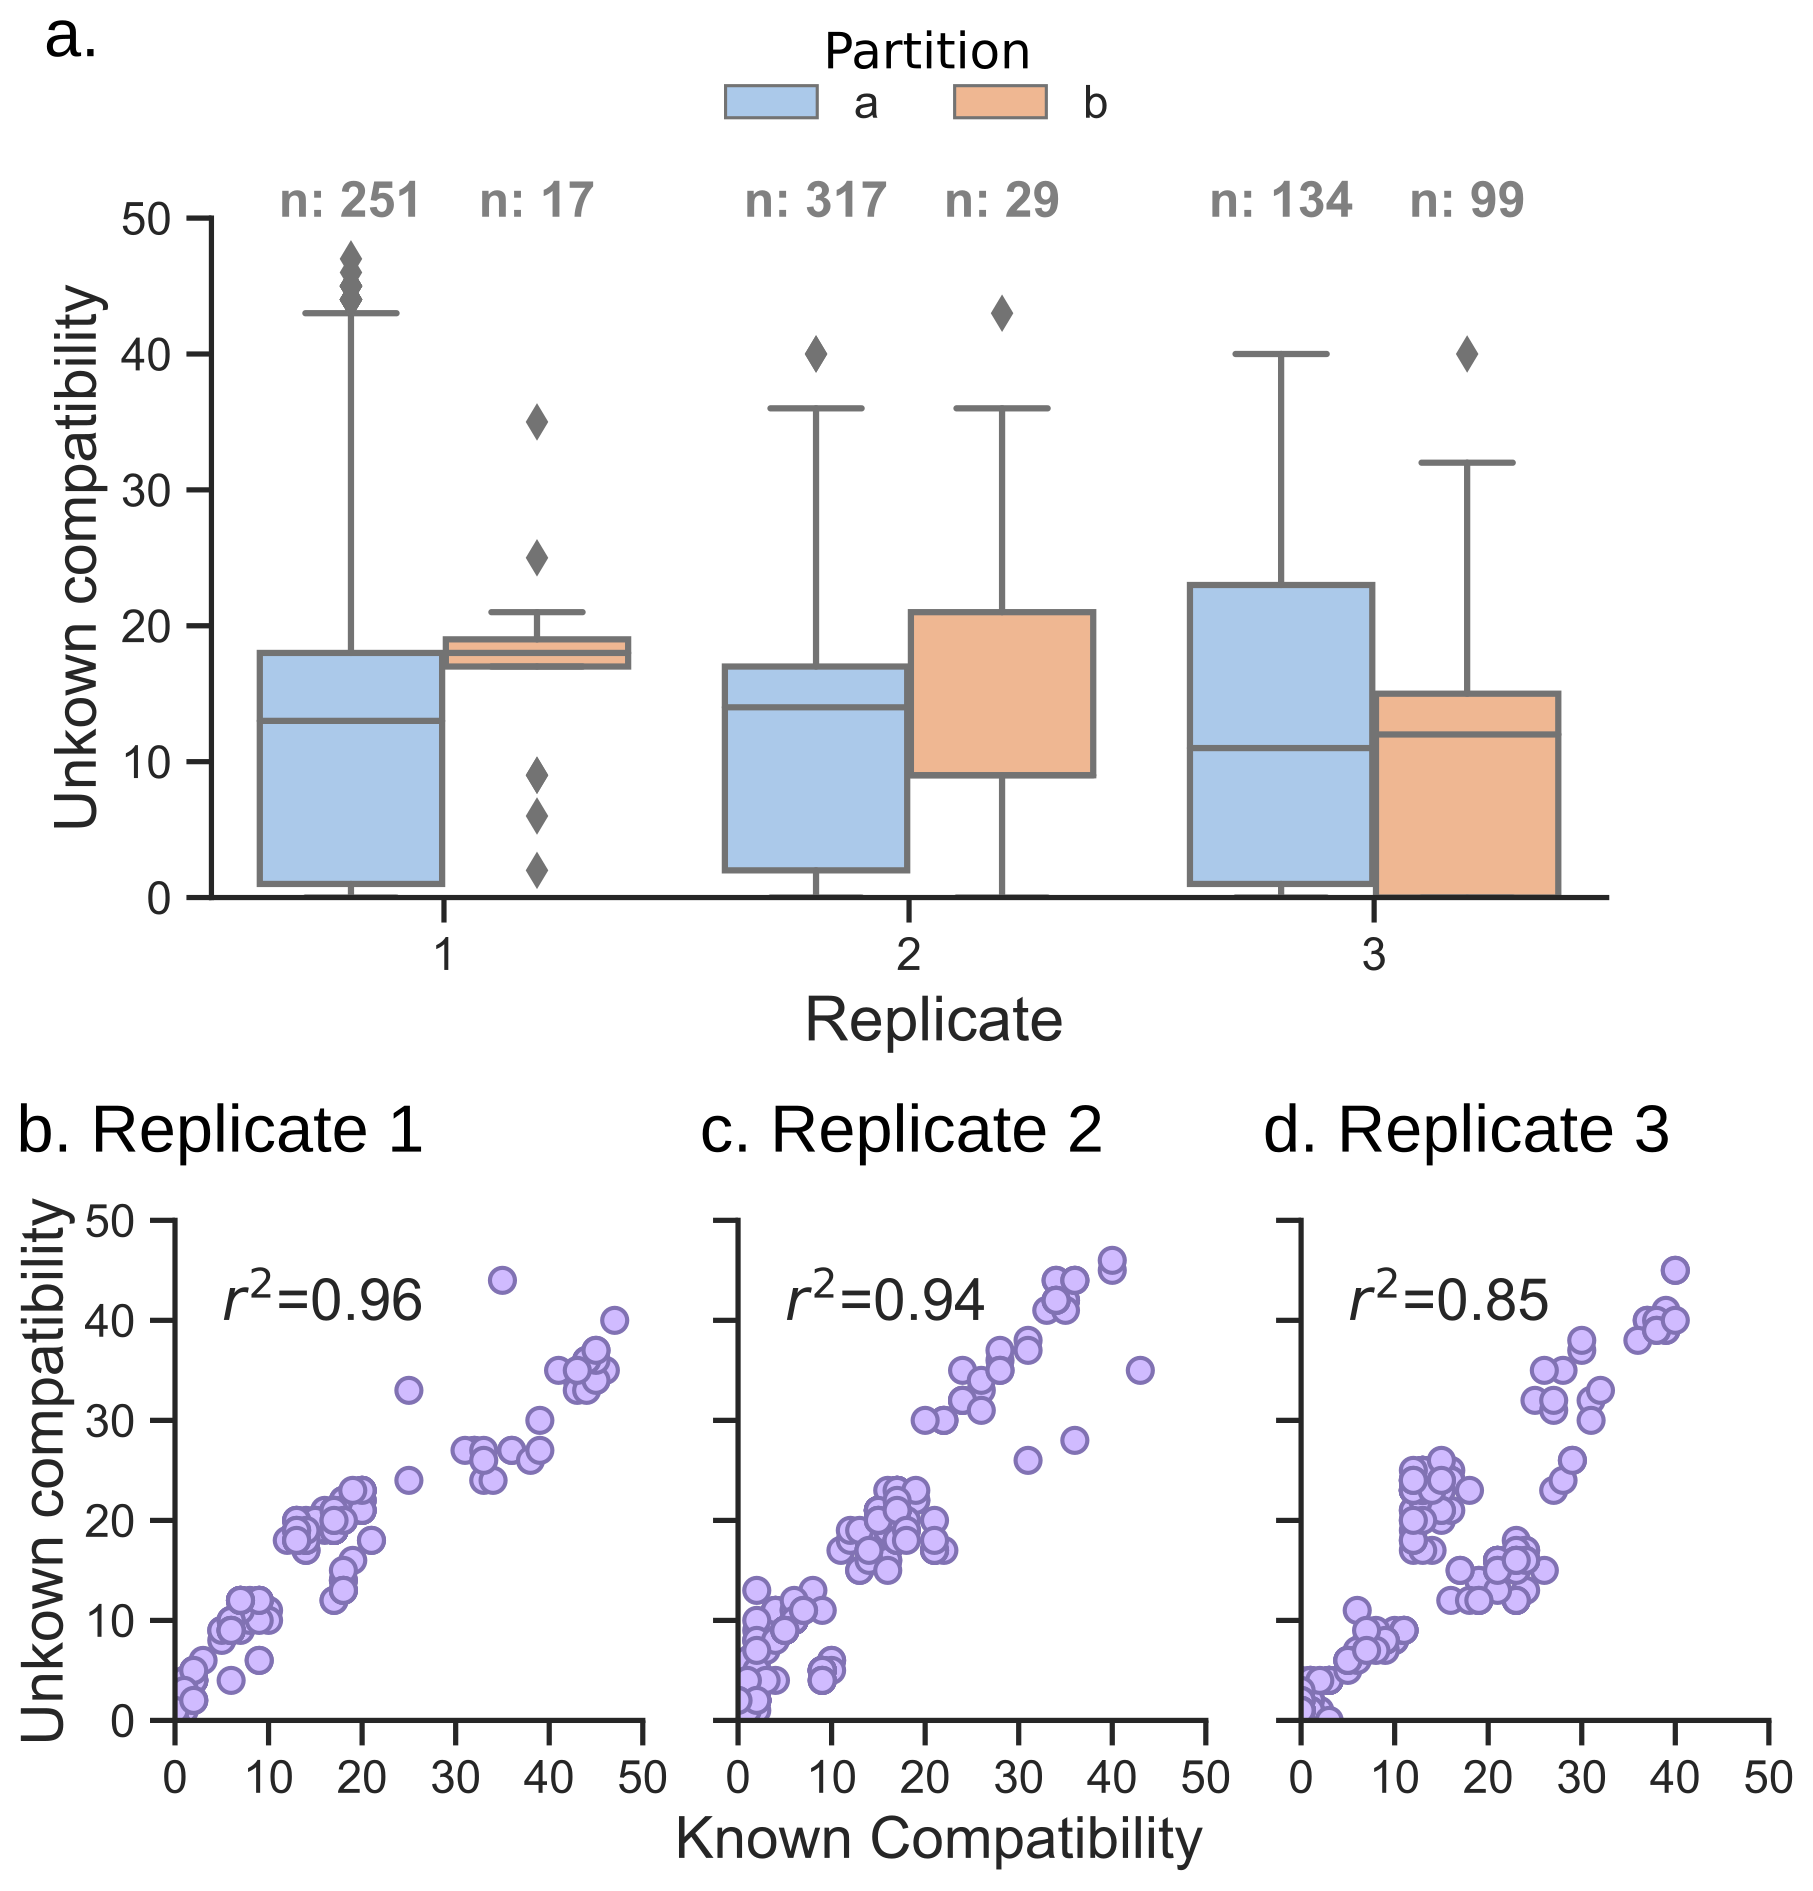
\includegraphics[width=.6\textwidth,keepaspectratio]{partitions.png}
    \caption[Compatibility towards unknown products]{Compatibility towards unknown products in 3 random even partitions of the product library. (a) Distribution of unknown compatibility, n corresponds to the number of designs in each case. (b-d) Comparison between unknown and known compatibility of each design for each replicate, $r^2$ is the Pearson correlation coefficient.}
    \label{fig7:partitions}
\end{figure}

\paragraph{Deletion reactions that remove major fermentation byproducts and alter redox metabolism have the highest contribution towards unknown compatibility}
%\paragraph{Reaction deletions that contribute the most towards unknown compatibility remove common fermentation byproducts followed by manipulations in redox metabolism}
% - Goal is to identify features of designs that contribute the most towards unknown compatibility
% - Describe approach
% - Conclude with LASER citation, this happen to be the intuitive strategies.

To identify the specific genetic intervention strategies that contribute to
the unknown compatibility of a design,  we defined the unknown compatibility contribution of deletion reaction $j$ ($ucc_j$) as follows:
\begin{equation}
    ucc_j=\frac{\sum\limits_{h\in\mathcal{H}_j} u_h}{|\mathcal{H}|}
\end{equation}
where $\mathcal{H}_j$ is the subset of designs from Pareto set ($\mathcal{H}$) containing deletion reaction $j$ and $u_h$ is the unknown compatibility of design $h$. %that corresponds to the compatibility towards modules not included as part of the ModCell-HPC input.
We computed $ucc$ for all 3 replicates and examined the top 10 sorted by mean value (Table~\ref{tab7:top10contrib}).
This revealed that the main contributors towards unknown compatibility are removal of major fermentative byproducts (lactate, ethanol, and acetate), indeed these are the strategies that repeat the most across the metabolic engineering literature,\citep{winkler2015} followed by manipulation of redox pathways (THD2pp, FLDR2, MDH) and metabolic branch points (TKT2, PPC).
Strain repurposing could be further explored with algorithms specialized for this task, e.g., by identifying module reactions in the unknown modules or using the existing strain as a starting point to identify genetic manipulations instead of a wild type strain.
In our analysis we have identified that high chassis compatibility and certain reaction deletions are indicators of compatibility towards unknown products.


\begin{table}[h]
    \caption[Top 10 reactions with highest unknown compatibility contribution]{Top 10 reactions sorted by mean unknown compatibility contribution ($ucc$) among replicates. }
    \centering
    \rowcolors{3}{gray!25}{white}
%\resizebox{1\textwidth}{!}{%
\begin{tabular}{llcccc}
\toprule
        &                                        &  \multicolumn{4}{c}{$ucc$}      \\
%\rowcolor{white}
%\rowcolors{2}{blue}{white}
%\cline{3-6}
\multirow{-2}{*}{ID} &    \multirow{-2}{*}{Name} &    R. 1 &    R. 2 &    R. 3                  &  Mean \\
\midrule
LDH\_D  &  D-lactate dehydrogenase & 13.2 & 10.5 & 11.9 & 11.9 \\
ALCD2x &  Alcohol dehydrogenase (ethanol) & 11.5 & 10.5 & 11.8 & 11.3 \\
PTAr   &  Phosphotransacetylase & 4.0 & 4.8 & 6.5 & 5.1 \\
ACALD  &  Acetaldehyde dehydrogenase (acetylating) & 4.5 & 2.8 & 2.9 & 3.4 \\
THD2pp &  NAD(P) transhydrogenase (periplasm) & 4.7 & 2.4 & 2.2 & 3.1 \\
ACKr   &  Acetate kinase & 3.8 & 2.2 & 1.7 & 2.6 \\
FLDR2  &  Flavodoxin reductase (NADPH) & 2.0 & 2.2 & 2.9 & 2.4 \\
TKT2   &  Transketolase & 2.6 & 2.0 & 2.5 & 2.4 \\
PPC    &  Phosphoenolpyruvate carboxylase & 2.3 & 2.2 & 2.5 & 2.3 \\
MDH    &  Malate dehydrogenase & 2.7 & 1.1 & 2.3 & 2.0 \\
\hline
\end{tabular}%}

    \label{tab7:top10contrib}
\end{table}

\section{Conclusions}
% - Develop modcell-hpc:
%       - What does it do
%       - Why is it useful
% - What do we find by applying modcell-hpc?
%
% - What are future challenges/directions?
%
% What are key aspects of the method developed here?
% What are key insights in the design of platform strains that result from applying the method?

% Some random points
%Notably, only a few genetic manipulations seem to be sufficient ...
%
%While current genetic engineering techniques may limit the validation of such system, due to the slow of product pathway construction and overexpression...
%
%- While growth coupling has advantages ...., such tight coupling, if implemented successfully, can not only be relevant at the pathway optimizataion stage, but also at the scaling up stage where loss of phenotype may occur. However, such design might be too strict and not be practical for all metabolites of interest. %(Make this claim on the basis of what results? Maybe only around 50\% of the library
%
%
%Remarkably, the proposed designs are consistent with isolated metabolic engineering strategies, reinforcing the potential for generalization of certain approaches.
%select good candidate products thorugh
%Further analysis at the metabolic strategies behind these designs revealed...
%
%%We identified a variety of designs, each compatible with dozens of products.

In this study we developed ModCell-HPC, a computational method to design modular platform strains compatible with hundredths of product synthesis modules.
We applied ModCell-HPC to a library of 161 products derived form the endogenous metabolism of \textit{E. coli} and used this same organism as a chassis.
This resulted in many Pareto optimal designs for the production of these molecules, from which we selected the smallest set of designs necessary to ensure any compatible product is present in at least one of them.
The designs feature strategies consistent with previous experimental studies aimed at optimizing production of a single product, reinforcing our confidence in the value of our simulations.
Remarkably, the strategies feature not only removal of major byproducts (e.g., lactate, ethanol), but also modification of key metabolic branch-points (e.g., deletion of TKT2 that alters flux between pentose phosphate and glycolysis pathways; or PPC, that alters flux from glycolysis towards the Krebs cycle).
We used growth-coupled to product formation as a target phenotype for each production module,
such platform strains can also enable high-throughput pathway engineering approaches, e.g., the chassis can be simultaneously combined with a library of modules to rapidly identify good candidate pathways through adaptive laboratory evolution.
We also used ModCell-HPC to design high compatibility platform strains to utilize different carbon sources, revealing the limitations of pentoses that might be addressed by redox cofactor engineering.
Finally, we used ModCell-HPC to investigate how existing strains might be repurposed towards products unknown at the time of design, and identified (known) compatibility and specific reaction deletions as important features of highly repurposable strains.
Overall, ModCell-HPC is an effective tool towards more efficient and generalizable design of modular platform strains that have recently captured the interest of metabolic engineers. \citep{nielsen2016}


%\singlespace



\section*{Supplementary Materials}
\begin{enumerate}%[label=Supplementary Material \arabic*, leftmargin=*]
    \item Supplementary text, figures, and tables. \label{sm:figures}
    \item Designs for selected parameters $\alpha=5,\,\beta=1$. \label{sm:designs}
    \item Computer programs used to generate the results of this study. \label{sm:code}
    %\item NOTE: what to do with reaction/metabolite abbreviations?
\end{enumerate}

